\documentclass[12pt,a4paper]{article}
\usepackage[utf8]{inputenc}
\usepackage{amsmath}
\usepackage[english]{babel}
\usepackage{amsfonts}
\usepackage{amssymb}
\usepackage{graphicx}
\usepackage{environ}
\usepackage{fancybox}
\usepackage[colorlinks,linkcolor=purple]{hyperref}
\usepackage{mathtools}
\usepackage{environ}
\usepackage{setspace}
\usepackage{wrapfig}
\usepackage{xcolor}
\usepackage{xparse}

\NewDocumentCommand{\framecolorbox}{oommm}
 {% #1 = width (optional)
  % #2 = inner alignment (optional)
  % #3 = frame color
  % #4 = background color
  % #5 = text
  \IfValueTF{#1}
   {\IfValueTF{#2}
    {\fcolorbox{#3}{#4}{\makebox[#1][#2]{#5}}}
    {\fcolorbox{#3}{#4}{\makebox[#1]{#5}}}%
   }
   {\fcolorbox{#3}{#4}{#5}}%
 }
 
 
\author{Olivier Cloux}
\title{Discrete Structure}
\date{Semestre 1}

\begin{document}


\newcommand{\combin}[2]{\begin{pmatrix}
#1\\
#2
\end{pmatrix}}
\newcommand{\somme}[3]{\ensuremath{\sum\limits_{#2}^{#1}\left(#3\right)}}
\newcommand{\produit}[3]{\ensuremath{\prod\limits_{#2}^{#1}\left(#3\right)}}
\newcommand{\limite}{\lim\limits_}
\newcommand{\evid}[1]{\textbf{\underline{#1}}}
\newcommand{\ninf}{\ensuremath{n \to \infty}}
\newcommand{\xinf}{\ensuremath{x \to \infty}}
\newcommand{\xo}{\ensuremath{x \to 0}}
\newcommand{\no}{\ensuremath{n \to 0}}
\newcommand{\xx}{\ensuremath{x \to x}}
\newcommand{\Xo}{\ensuremath{x_0}}
\newcommand{\E}{\ensuremath{\mathbb{E}}}
\newcommand{\A}{\ensuremath{\mathbf{A}}}
\newcommand{\R}{\ensuremath{\mathbb{R}}}
\newcommand{\N}{\ensuremath{\mathbb{N}}}
\newcommand{\Z}{\ensuremath{\mathbb{Z}}}
\newcommand{\Q}{\ensuremath{\mathbb{Q}}}
\newcommand{\rtor}{\ensuremath{\R \to \R}}
\newcommand{\ts}{\textsuperscript}
\newcommand{\bo}{\textbf}
\newcommand{\Ngo}{\ensuremath{\mathbb{N}_{\geq 0}}}
\newcommand{\Example}{\underline{Example}}
\newcommand{\Definition}{\underline{Definition}}
\newcommand{\f}{\ensuremath{f} }
\newcommand{\combi}[2]{\ensuremath{\begin{pmatrix} #1 \\ #2 \end{pmatrix}}}

\NewEnviron{boiteV}[1]{
\begin{center}
\framecolorbox{red}{white}{\begin{minipage}{#1\textwidth}
\BODY
\end{minipage}}
\end{center}}

\NewEnviron{boite}[1][0.9]{
\begin{center}
	\framecolorbox{red}{white}{
		\begin{minipage}{#1\textwidth}
  			\BODY
	\end{minipage}
	}
\end{center}
}


\maketitle
\tableofcontents
\setstretch{1.6}

\section{Introduction}
\subsection{Recommended Book} Lay Roser, 7\ts{th} Edition.\\
\subsection{Grade} Max $\{\frac{Homework}{10} + 3\cdot\frac{Midterm}{10} + 6\cdot\frac{Final}{10} ; Final\}$\\
\subsection{Purpose}
\begin{enumerate}
	\item Review some basic math facts
	\item Algorithm thinking
	\item Solution scales
\end{enumerate}
\subsection{Working on :}
\begin{enumerate}
	\item \textit{logic} - how to prove things
	\item algorithm - to do things
	\item counting - complexity of algorithms
	\item probability - what to expect
\end{enumerate}
\subsection{Examples}
\begin{itemize}
	\item[First example :] If for two integers m and n, their product $m\cdot n$ is odd, then both m and n are odd.

	\underline{Proof :}If m is even then, regardless of n, $m\cdot n$ is even. Hence, since we know by assumption that $m\cdot n$ is odd, it follows that n is odd. Some argument applies to n.

	\item[Second example :] \underline{Claim :} For all integers k, and for all integers m and n, if m+n $\geq$ 2k, then either m $\geq$k, or n $\geq$ k.

	\underline{Proof :} Assume not (assume that conclusion is false). 		Then there exists k, m, n $\in$ $\pmb{\mathbb{Z}}$ so that $m < k$ and $n < k$ but $m+n \geq k$. But if $, < k$ and $n < k$, we can conclude :
	\\
	$m < k$\\
	$n < k$\\
	$m + n < 2k \rightarrow$ Contradiction !
\end{itemize}

\section{Propositional Logic}


\subsection{Definition}
\begin{boite}
\underline{Definition :}
	A \textit{proposition} is a declarative sentence,a sentence declaring/stating a fact.
	\\ A proposition can either be true (T) or false (F), but not both !
\end{boite}
\underline{Examples :}\\
"2+3=5" is True, "Today is tuesday" is True but "This course is boring" is obviously False.

\subsection{Logical operates}
\begin{itemize}
	\item[$\wedge$] "and" - Conjunction
	\item[$\vee$]  "or" - Disjunction
	\item[$\neg$] "it is not the case that..." - Negation
	\item[$\bigoplus$] "Xor"
	\item[$\rightarrow$] "if...then" - Implies, Conditional
	\item[$\leftrightarrow$] "if and only if (iff)" - Bi-conditional
\end{itemize}
\underline{Note :} we use p,q,r,s,t to denote propositions.\\
by combining propositions, via logical operators we got compound propositions (just a proposition, but more "complicated").

\subsection{Truth tables}
\begin{center}
\begin{tabular}{cc|cccccc}
p & q & $\neg p$ & $p \wedge q$ & $p \vee q$ & $p \bigoplus q$ & $p \rightarrow q$ & $p \leftrightarrow q$ \\ 
\hline 
1 & 1 & 0 & 1 & 1 & 0 & 1 & 1 \\ 
1 & 0 & 0 & 0 & 1 & 1 & 0 & 0 \\ 
0 & 1 & 1 & 0 & 1 & 1 & 1 & 0 \\ 
0 & 0 & 1 & 0 & 0 & 0 & 1 & 1 \\ 
\end{tabular} 
\end{center}
\subsection{Examples of logical equivalence}
\subsubsection{First example :$p \rightarrow q \equiv \neg p \vee q$}
\begin{center}
	\begin{tabular}{cc|cc}
		p & q & $\neg$p & $\neg$p$\vee$q\\
		\hline
		T&T&F&T\\
		T&F&F&F\\
		F&T&T&T\\
		F&F&T&T\\
	\end{tabular}
\end{center}
\subsubsection{Second example : $(p \rightarrow q) \wedge (q \rightarrow p) \equiv p \leftrightarrow q$}
\begin{center}
	\begin{tabular}{cc|ccc}
		p & q & p$\rightarrow$q & q$\rightarrow$p & 							(p$\rightarrow$q)$\wedge$(q$\rightarrow$p)\\
		\hline
		T&T&T&T&T\\
		T&F&F&T&F\\
		F&T&T&F&F\\
		F&F&T&T&T\\
	\end{tabular}
\end{center}

\subsection{Laws}
\begin{itemize}
	\item[De Morgan's Law] $\neg$(p $\wedge$ q) $\equiv$ ($\neg$p) $\vee$ ($\neg$q)
	\newline $\neg$(p $\vee$ q) $\equiv$ ($\neg$p) $\wedge$ ($\neg$q)

	\item[Identity law] p$\wedge$\bo{T} $\equiv$ p
	\newline p$\vee$\bo{F} $\equiv$ p

	\item[Domination law] p$\vee$\bo{T} $\equiv$ \bo{T}
	\newline p$\wedge$\bo{F} $\equiv$ \bo{F}

	\item[Idempotent law] p$\vee$p $\equiv$ p
	\newline p$\wedge$p $\equiv$ p

	\item[Double negation law] $\neg(\neg p) \equiv p$

	\item[Commutating law] $p \vee q \equiv p$
	
	\item[Asociativity law] $(p \vee q) \vee r \equiv p \vee (q \vee r)$
	\newline$(p \wedge q) \wedge r \equiv p \wedge (q \wedge r)$
	
	\item[Absorption law]$p \vee (p \wedge q) \equiv p$
	\newline $p \wedge (p \vee q) \equiv p$
	
	\item[Distributive law]$p \vee (q \wedge r) \equiv (p \vee q) \wedge (p \vee r)$
	\newline $p \wedge (q \vee r) \equiv (p \wedge q \vee (p \wedge r)$
	
	\item[Negation Law] $p \vee \neg p \equiv \bo{T}$
	\newline $p \wedge \neg p \equiv \bo{F}$
\end{itemize}
\subsubsection{De Morgan's law}
\begin{center}
	\begin{tabular}{cc|ccccc}
		p & q & p$\wedge$q & $\neg$(p$\wedge$q) & $\neg$p & $\neg$q & 			($\neg$p)$\vee$($\neg$q)\\
		\hline
		T&T&T&F&F&F&F\\
		T&F&F&T&F&T&T\\
		F&T&F&T&T&F&T\\
		F&F&F&T&T&T&T\\
	\end{tabular}
\end{center}
as we can see, the 4\ts{th} and the 7\ts{th} columns are the same $\rightarrow$ they are logically equivalent.
\subsubsection{Example (use of laws)}
\underline{Claim :} $\neg(p\vee (\neg p\wedge q)) \equiv \neg p \wedge  \neg q$ \\
\underline{Proof :}\\
$\neg(p\vee (\neg p\wedge q))$\\
$\equiv \neg p \wedge (\neg (\neg p \wedge q))$ De Morgan's Law\\
$\equiv \neg p \wedge (\neg (\neg p) \vee \neg q)$ De Morgan's Law\\
$\equiv \neg p \wedge (p \vee \neg q)$ Double Negation Law\\
$\equiv (\neg p \wedge p) \vee (\neg p \wedge \neg q)$ Distributive Law\\
$\equiv \bo{F} \vee (\neg p \wedge \neg q)$\\
$\equiv \neg p \wedge \neg q$

\subsection{Predicate}
\begin{center}
	\fbox{\begin{minipage}{0.9\textwidth}
		\underline{Definition :}
		\\ A "formula that involves some variables. These variables come from a domain, call D, and this domain must be specified
		\\
		For example : P(x) = "x $\geq$ 3". P(x) is a predicate.\\

		If you take a predicate and fix the values, then it becomes a \textit{proposition} with a definite truth value\\
		For example : P(4) = "4 $\geq$ 3"  T, but P(2) = "2$\geq$3  F. P(..) is a proposition.
	\end{minipage}} 
\end{center}

\subsection{Quantifiers}
\begin{itemize}
	\item[Universal quantifier :] $\forall$x P(x), read "for all x (in the domain) P(x)". \\
	\underline{Notes :} 
	\begin{itemize}
		\item There is a domain that must be specified.
		\item $\forall$x P(x) is a proposition, with a truth value T if and only if for all values x in the domain, P(x) has truth value T.		
		\item If the domain D is finite D=\{$x_1$, $x_2$,...$x_n$\} $\forall$x P(x) $\equiv$ P($x_1$) $\wedge$ P($x_2$) $\wedge$... P($x_n$).
	\end{itemize} 
	
'	\item[Existential quantifier :] $\exists$x P(x) . Read "there exists (in the domain) a value x so that P(x)"\\
	\underline{Notes :}	
	\begin{itemize}
		\item $\exists$x P(x) is a proposition, with truth value T if and only if there exists \underline{at least} one element x in the domain so that P(x) has truth value T.
		\item If D is finite then, D=\{$x_1$, $x_2$,...$x_n$\}. $\exists$x P(x) $\equiv$ P($x_1$) $\vee$ P($x_2$) $\vee$... P($x_n$).
	\end{itemize}
\end{itemize}

\subsubsection{Examples}
\begin{itemize}
\item P(x) = "x $\geq$ 3", D = $\pmb{\mathbb{R}}$\\
$\forall$x P(x)  F (P(2) is false)\\
$\exists$x P(x)  T (P(4) is true)
\item P(x, y) = "x $\geq$ 3$y^2$"\\
$\exists$x$\exists$y P(x, y)  T  (P(4, 1) is true)\\
$\forall$x$\forall$y P(x, y)  F  (P(1, 1) is a counterexample)\\
$\forall x (\exists y  P(x, y)$ F  ($P(-1 y) = "-1 \geq 3\times y^2"$\\
$\exists y \forall x P(x, y)$    F\\
$\exists x \forall y P(x,y)$   F\\
$\forall y \exists x P(x, y)$  T
\end{itemize}
\fbox{
\begin{minipage}{0.9\textwidth}
   \underline{Note :} $\forall x \exists y P(x, y) \neq \exists y \forall x P(x, y)$. It implies that $\exists y \forall x P(x, y) \rightarrow \forall x \exists y P(x, y)$
\end{minipage}
}

\subsubsection{Negation of Quantifiers}
\begin{itemize}
	\item $\neg (\forall x P(x)) \equiv \exists x \neg P(x)$
	\item $\neg (\exists x P(x)) \equiv \forall x \neg P(x)$
	\item $\neg (\forall x \forall y, P(x,y)) \equiv \exists \neg (\forall y, P(x,y)) \equiv \exists x \exists y \neg P(x,y)$
\end{itemize}

\underline{Proof :} $\neg (\forall x P(x))$ is true iff $\neg (\neg (\forall x P(x)))$ is false, which means that $\forall x, P(x)$ is false, which means that there exists at least one value in the domain so that $P(x)$ is false, or equivalently, that $\neg P(x)$ is true. The last can be written as $\exists x \neg P(x)$.

\subsubsection{Application to our original example}
Let us go back to one of our initial examples. D = $\pmb{\mathbb{{Z}}}$
p="$\forall m,n,k|(m+n \geq 2k)  \rightarrow ((m \geq k) \vee (n \geq k))$"
Proving this statement means hat we show that p has truth value \bo{T}. This is equivalent to show that $\neg p$ has truth value \bo{F}. 

$P \overset{?}{=} \bo{T}$  $\neg P \overset{?}{=} F$\\
$\neg (\forall m, n, k | (m+n \geq 2\cdot k) \rightarrow ((m \geq k) \vee (n \geq k))$ \\$\equiv \exists m, n, k | \neg (m+n \geq 2\cdot k) \rightarrow ((m \geq k) \vee (n \geq k))$ \\
\\
$\ulcorner$ Simplified :
\\$ \neg (p \rightarrow q)$\\
$\equiv \neg (\neg  p \vee q)$\\
$\equiv \neg (\neg p) \wedge \neg q$\\
$\equiv p \wedge \neg q $  $\lrcorner$\\
\\
$\equiv \exists m, n, k| (m+n \geq 2\cdot k) \wedge \neg (((m \geq k) \vee (n \geq k))$\\
$\equiv \exists m, n, k| (m+n \geq 2\cdot k) \wedge (m < k) \wedge (n < k)$\\
$m < k$\\
$n < k$\\
$m+n < 2\cdot k \Rightarrow$ Is false, so $\neg P$ is false, so $P$ is true\\
\underline{It was a proof by \textit{contradiction}.} Just negate the original proposition, and the answer is opposite of the outcome.

$p \rightarrow q \equiv q \vee \neg p \equiv \neg q \rightarrow \neg p$\\
\begin{center}
\fbox{
\begin{minipage}{0.5\textwidth}
\begin{equation*}
p \rightarrow q \equiv \neg q  \rightarrow \neg p
\end{equation*}
\end{minipage}}
\end{center}

So, an equivalent way to prove :\\
$p = "m+n \geq 2\cdot k"$\\
$q = "(m\geq k) \vee (n \geq k)"$. To know if $p \rightarrow q$ is true, we can  see if \\
$\neg q \rightarrow \neg p$ is true, with\\
$\neg p = "(m < k) \wedge (n < k)"$\\
$\neg q = m+n < 2\cdot k$ 

\subsubsection{Unique solution}
$\exists x P(x)$, read "There exists at least one value x so that P(x)\\
$\exists ! x P(x)$, read There exists a unique x so that P(x).

\subsubsection{Negation of unique solution}
What is $\neg (\exists ! x P(x))$ ?\\
$\neg (\exists ! x P(x) \equiv \neg (\exists x$ [TROU]

\subsubsection{Summary}
\begin{itemize}
	\item[Predicates]
	\item 
	\begin{itemize}
		\item[P(x)] x variable, $\in$ D
		\item[P(1)] Proposition
	\end{itemize}
	\item[Quantifiers]
	\item 
	\begin{itemize}
		\item $\exists$ x P(x)
		\item $\forall$ P(x)
		\item $\exists !$ x P(x)
		\item $\forall x \geq$  P(x)
	\end{itemize}
\end{itemize}

Examples : F(x,y) = "x can fool y". 
So :
\begin{itemize}
	\item $\forall x$ F(x, Jim)= Everybody can fool Jim.
	\item $\forall x$ F(Evelyn, x) = Evelyn can fool everybody.
	\item $\forall x \exists y$ F(x, y) = Everybody can fool somebody.
	\item $\exists y \forall x$ F(x, y) = There exists a person who can be fooled by everyone.
	\item $\neg$($\exists x$F(x, x)) = Nobody can fool himself.
	\item ($\exists ! x$ F(x, x)) $\wedge$ F(Penny, Penny) = Only Penny can fool herself.
\end{itemize}

\subsection{Rules of Inference}
p $\rightarrow$ q. p is an assumption, and q is the desired conclusion. "prove" means to show that p $\rightarrow$ q has truth value T.\\
\underline{Example :}
\begin{enumerate}
	\item If Eric does not have 8 legs, then Eric is not a insect.
	\item Eric is an insect.
\end{enumerate}
\underline{Question :} Can we conclude that Eric has 8 legs ?\\
\\
\underline{Formalize :} \\
p = "Eric does not have 8 legs"\\
q = "Eric is not an insect". 
\begin{enumerate}
	\item $p \rightarrow q$ 
	\item $\neg q$
\end{enumerate}
\underline{Desired conclusion :} $\neg$p. \\
This is equivalent to asking if $((p \rightarrow q) \wedge \neg q) \rightarrow \neg q$ has always truth value \bo{T}. This is called a \underline{tautology}
\begin{center}
\begin{tabular}{cc|ccccc}
		p & q & $\neg p$ & $\neg q$ & $p \rightarrow q$ & $(p \rightarrow q) \wedge \neg q$ & $((p \rightarrow q) \wedge \neg q) \rightarrow \neg p$\\
		\hline
		T&T&F&F&T&F&T\\
		T&F&F&T&F&F&T\\
		F&T&T&F&T&F&T\\
		F&F&T&T&T&T&T\\
	\end{tabular}
\end{center}

\subsubsection{The rules :}
%encore à modofier. piste: inferrule. mais comment installer ?
\begin{itemize}
	\item[Modus tollens] (p $\rightarrow$ q, $\neg$q), $\neg$p
	\item[Modus ponens] (p, p $\rightarrow$ q), q
	\item[Simplification] (p $\wedge$ q), p
	\item[Addition rule] (p), p $\vee$ q
	\item[Conjuction] (p, q), p $\wedge$ q
	\item[Hypothetical syllogism] ($p \rightarrow q, q \rightarrow r$), p $\rightarrow$ r
	\item[Disjunctive syllogism] ($p \vee q, \neg p$), q
	\item[Resolution] ($p \vee q, \neg p \vee r$), $q \vee r$
	\item[Universal generalizaton] (P(x) for all x $\in$ D), $\forall x P(x)$
	\item[Universal specialization] ($\forall x P(x)$), P(d) for any d $\in$ D
	\item[Existential generalization] (P(d) for some d $\in$ D), $\exists x P(x)$
	\item[Existention specializazion] ($\exists x P(x)$), P(d) for some d $\in$ D
\end{itemize}
\subsubsection{Proof example}
\underline{Assumptions}

\begin{enumerate}
	\item Someone in this class visited the US.
	\item Anybody who visited the US likes hamburgers.
\end{enumerate}
\underline{Desired conclusion :} There is someone in this class who likes hamburgers.\\
\\
\underline{Predicates :} 

\begin{itemize}
	\item C(x) = "x is in this class".
	\item V(x) = "x visited the US".
	\item L(x) = "x likes hamburgers"
\end{itemize}
\underline{Writing our assumptions in mathematical language}
\begin{enumerate}
	\item $\exists x (C(x) \wedge V(x))$
	\item $\forall x ( V(x) \rightarrow L(x))$
\end{enumerate}
\underline{Writing our desired conclusion in mathematical language}\\
\\
$\exists x (C(x) \wedge L(X))$\\
\\
\underline{Solving :}
\begin{enumerate}
	\item $\exists x (C(x) \wedge V(x))$
	\item $\forall x ( V(x) \rightarrow L(x))$ (those are our assumptions)
	\item $C(d) \wedge V(d)$ (From 1, using exist. simplif., d, D some suitable elements.
	\item C(d)
	\item V(d) (4 and 5 from 3, using simplification rule)
	\item $V(d) \rightarrow L(d)$ (from 2, using universal specialization).
	\item L(d) (using 5\&6 and modus ponens)
	\item $C(d) \wedge L(d)$ (usig 4 and 7 and conjunction rule).
	\item $\exists x (C(x) \wedge L(x))$ (using 8 and existential generalization).
\end{enumerate}

\subsubsection{So far we have seen}
\begin{enumerate}
	\item[Direct proof] P $\rightarrow$ q. Start with assumptions, apply inference rules, at some point to get q (example : hamburger proof)
	\item[Proof by contraposition :] $p \rightarrow q \equiv \neg q \rightarrow \neg p$. Now start with $\neg q$ ; use rules of inference to arrive at $\neg p$.
	\item[Proof by contradiction] "$p \rightarrow q$" is true, so $\neg (p \rightarrow q)$ is false ($\equiv \neg (\neg p \vee q) \equiv p \wedge \neg q$
\end{enumerate}

\section{Sets}
\begin{center}
\fbox{
\underline{Definition :} A set is an unordered collection of distinct objects.}
\end{center}
$A = \{2,3,5,7,11\}$ all primes less than 13 = $\{3,2,11,7,5,3\}$. 3 is a membre (an element) of A ($3 \in A$).\\
$B = \{0,1,2,3,...,100\}$ all integers between 0 and 100

\subsection{Set builder notation}
S = $\{x : P(x)\} = \{x| P(x)\}$ (to define the domain/universe). $x \in \mathbb{N}$. P(x) is a predicate.\\
A = $\{x \in \mathbb{Z} :$ (x is prime) $\wedge$ (x $\leq$ 13)$\}$
B= $\{x : (x \in \mathbb{Z}) \wedge (0 \leq x \leq 100)\}$

\subsection{Common Sets}
\begin{itemize}
	\item[$\mathbb{N}$] natural numbers, non negative integers. 0 could or not be included.
	\item[$\mathbb{Z}$] Integers
	\item[$\mathbb{Q}$] Rationals
	\item[$\mathbb{R}$] Reals
	\item[$\mathbb{C}$] Complex numbers
\end{itemize}

\subsubsection{Cardinality}
$|A|$ or $\#A$ represents the numbers of elements in the set. For example, $|A| = 5$, and $\|B| = 101$. But those are finite sets.\\
$|\mathbb{N}| =  |\mathbb{Z}| = \mathbb{Q}| = "\infty"$ are infinite sets.
$|\mathbb{R}| =  |\mathbb{C}| = \infty \neq |\mathbb{N}|$. These are not the same infinity.

\subsubsection{Some more notions}
\begin{itemize}
	\item $\{\} = \emptyset$
	\item $\{\bigtriangleup\}$ = singleton (a single and alone element).
	\item A = B represents equality between two sets. (so ($A \subseteq B) \wedge ( B \subseteq A))$
	\item $A \subseteq B$ = A is a subset of B. Means that $\forall x ( x \in A \rightarrow x \in B)$
	\item $\emptyset \subseteq S$. S any set. $\forall x ( x \in \emptyset \rightarrow x \in S)$.
	\item $S \subseteq S$. S any set as well. $\forall x ( x \in S \rightarrow x \in S)$
	\item $A \cup B$ union. $A \cup B = \{x : x \in A \vee x \in B\}$.
	\item $A \cap B$ intersection. $A \cap B = \{x : x \in A \wedge x \in B\}$.
	\item $A \setminus B$ A minus B.$A \setminus B = \{x : x \in A \wedge x \not\in B\}$.
	\item $\overline{A}$ complement of A. = $\{x : \neg (x \in A)\}$
	\item A $\bigtriangleup B$ Symmetric difference. $A \bigtriangleup B = \{x : x \in A \bigoplus x \in B\}$.
	\item P(A) powerset of A is the set that consists of all subsets of A (see further). 
	\item $\overline{(A \cup B)} = \overline{A} \cap \overline{B}$
	\item $\overline{(A \cap B)} = \overline{A} \cup \overline{B}$
	\item (we can say $\cap$ is like $\wedge$ and $\cup$ is like $\vee$
\end{itemize}
\paragraph{Question : How can we prove such identities ?\\ $\overline{A \cup B} = \overline{A} \cap \overline{B}$\\}
There are 3 possible ways :
\begin{enumerate}
	\item By membership tables
	\item $...\subseteq...\cap...\supseteq...$
	\item direct way.
\end{enumerate}

\begin{enumerate}
	\item Table of truth \begin{center}
	\begin{tabular}{cc|ccccc}
		A & B & $\overline{A}$ & $\overline{B}$ & $A \cup B$ & $\overline{A \cup B}$ & $\overline{A} \cap \overline{B}$ \\ 
		\hline
		 T & T & F & F & T & F & F \\ 
		 T & F & F & T & T & F & F \\ 
		 F & T & T & F & T & F & F \\ 
		 F & F & T & T & F & T & T \\ 
	\end{tabular}
	\end{center}
\item Logical equivalences\\ $\overline{A \cup B} \subseteq$ (and $\supseteq$ too) $\overline{A} \cap \overline{B}$ \\
$x : x \in \overline{A \cup B}$\\
$\leftrightarrow \neg (x \in A \cup B)$\\
$\leftrightarrow \neg (x \in A \vee x \in B)$\\
$\leftrightarrow x \not \in A \wedge x \not \in B$\\
$\leftrightarrow x \in \overline{A} \wedge x \in \overline{B}$\\
$\leftrightarrow x \in \overline{A} \cap \overline{B}$\\

\item With equalities :\\
$\overline{A \cup B} = \{x : x \not\in (A \cup B)\}$\\
$= \{x : x \not \in A \cup B\}$\\
$= \{x : \neg (x \in A \cup B)\}$\\
$= \{x : \neg ("x \in A" \vee "x \in B")\}$\\
$= \{x : \neg (x \in A) \wedge \neg (x\in B)\}$\\
$= \{x : x \in \overline{A} \wedge x \in \overline{B}\}$\\
$= \overline{A} \cap \overline{B}$
\end{enumerate}

\subsection{Powerset}
\begin{center}
\fbox{\begin{minipage}{0.9\textwidth}
\underline{Definition : } P(A) Powerset of A is the set that consists of all subsets of A.
\end{minipage}}
\end{center}
\underline{Example :} $A = \{1,2,3\}$ (\underline{note :} Is A is finite, then $|P(A)| = 2^{|A|}$)\\
$P(A) = \{\emptyset, \{1\}, \{2\}, \{3\}, \{1,2\}, \{1,3\}, \{2,3\}, \{1,2,3\}\}$\\
$\emptyset = \{\}$\\
$P(\emptyset) = \{\emptyset\} \neq \emptyset$. $\emptyset \subseteq A$ always true !\\
$P(P(\emptyset)) = \{\emptyset, \{\emptyset\}\}$. $|P(A)| = 2^{|A|} = 2^0 = 1$\\
$|P(P(\emptyset))| = 2$

\subsection{Cartesian Product}
A, B set. $A \times B = \{(a,b) : a \in A \wedge b \in B\}$\\
Example : $A = \{1,2\}, B = \{\bigtriangleup, \bigcirc, \boxdot\}$\\
$A \times B = \{(1,\bigcirc), (1,\boxdot), (1,\bigtriangleup), (2,\boxdot), (2,\bigcirc), (2,\bigtriangleup)\}$\\
$|A \times B| = |A| \cdot |B|$\\
$A \times B \times C = \{(a,b,c) : a \in A, b \in B, c \in C\}$

\subsection{Venn diagram}
%[DESSIN 1]

\subsection{Set identities}
\begin{enumerate}
	\item $A \cup \overline{A} = U$ \\
	$\{x : x \in A\} \cup \{x : x \not \in A\} = \{x : x \in A \vee \neg (x \in A))\} = \{x \in U\}$
	\item $B \cap (A \cup \overline{A}) = (B \cap A) \dot{\cup} (B \cap \overline{A})$\\
	 i.e. $(B \cap A) \cap (B \cap \overline{A}) = \emptyset$ 
	\item $A \cup B = A \dot{\cup} (B \setminus A) \Rightarrow A \cap (B \setminus A) =\emptyset$ \\
	$=\{x : (x \in A) \wedge (x \in B \wedge x \in \overline{A})\}$\\
	$=\{x : (x \in B) \wedge (x \in A) \wedge (x \in \overline{A})\} = \emptyset$
	\item $B/A = B \cap \overline{A}$\\
	$=\{x : x \in B \wedge x \not \in A\} = \{x : (x \in B) \wedge (x \in  \overline{A})\}$
\end{enumerate}
\subsection{Inclusion and exclusion principle}
\underline{Claim :} Let A and B be two sets. $|A \cup B| = |A| + |B| - |A \cap B|$\\
\\
\underline{Intuition :} Venn's diagram\\%[DESSIN 2], diagrammes de Venn
\\
\underline{Aim :} Prove this counting identity.\\
\\
\underline{Special case} : Let A and B be two sets so that $A \cap B = \emptyset$. So, $|A \cup B| = |A| + |B|$ is true. We don't have the tools to prove it now, the diagrams and intuitions are enough.\\
\\
\underline{Proof of general case :} From 3, $A \cup B = A \dot{\cup} (B\setminus A) \Rightarrow A \cap (B\setminus A) = \emptyset$\\
Use special case to solve :\\
$|A \cup B| = |A \dot{\cup} (B\setminus A)| = |A| + |B \setminus A|$\\
$B \setminus A = B\cap \overline{A}$\\
$B = B \cap U = (B \cap A) \dot{\cup} (B \cap \overline{A})$\\
$|B| = |(B \cap A) \dot{\cup} (B \cap \overline{A}| = |B \cap A| + |B \cap \overline{A}|$\\
$|B \cap \overline{A}| = |B| - |B \cap A|$

\subsubsection{Example :}
$A = \{n \in \mathbb{Z} : (0 \leq n \leq 100) \wedge 5/n \}$ = \{, 5, 10, 15, ..., 100\}\\
$B = \{n \in \mathbb{Z} : (0 \leq n \leq 100) \wedge 7/n \}$ = \{0, 7, 14, 21, ...\}\\
Using the formula $|A \cup B| = |A| + |B| - |A\cap B|$. At this point, we know that $|A| = 21$, $|B| = 15$\\
$A \cap B = \{n \in \mathbb{Z} : (0 \leq n \leq 100) \wedge (5/n) \wedge (7/n) \}$, and as $(5/n) \wedge (7/n) \equiv 35/n \rightarrow A \cap B = \{ 0, 35, 70\} \rightarrow |A\cap B| = 3$\\
$|A \cup B| = |A| + |B| - |A\cap B| = 21 + 15 - 3 = \underline{33}$

\subsubsection{The 3 sets case :}
And what about $|A \cup B \cup C|$ ? The method to find it, is to substitute $D$ to $B \cup C$. The steps so become :\\
$|A \cup B \cup C| = |A \cup D| = |A| + |D| - |A \cap D| = |A| + |B \cup C| - |A \cap (B \cup C)|$\\
$=|A| + |B| + |C| -|B \cap C| - |(A \cap B) \cup (A \cap C)|$

\begin{center}
\fbox{\begin{minipage}{0.9\textwidth}
$|A \cup B \cup C| = |A| + |B| + |C| - |A \cap B| - |A \cap C| -|B \cap C| + |A \cap B \cap C|$
\end{minipage}}
\end{center}

\newpage
\subsection{Functions }
Two sets A and B.
\begin{center}
\fbox{\begin{minipage}{0.9\textwidth}\underline{Definition :} A function, call it f, from A to B is on assignment of a unique element of B to each element of A. \underline{We write} f(a) = b. We say that f maps a to b.
\end{minipage}}
\end{center}

f: $A \rightarrow B$. A is the domain, and B the co-domain.\\
\underline{Range of f } = $\{b \in B : \exists a \in A, f(a) = b\} \subseteq B$.\\
 We say that $b$ is the \underline{image} of $a$ by $f$. We call $a$ \underline{a pre-image} of $b$.

\subsubsection{Composition}
$f: A \rightarrow B$\\
$g: B \rightarrow C$\\
$h = g \circ f : A \rightarrow C$\\
$h(a) = g(f(a))$\\
attention : in most case, $f \circ g \neq g \circ f$

\subsubsection{Properties of functions :}
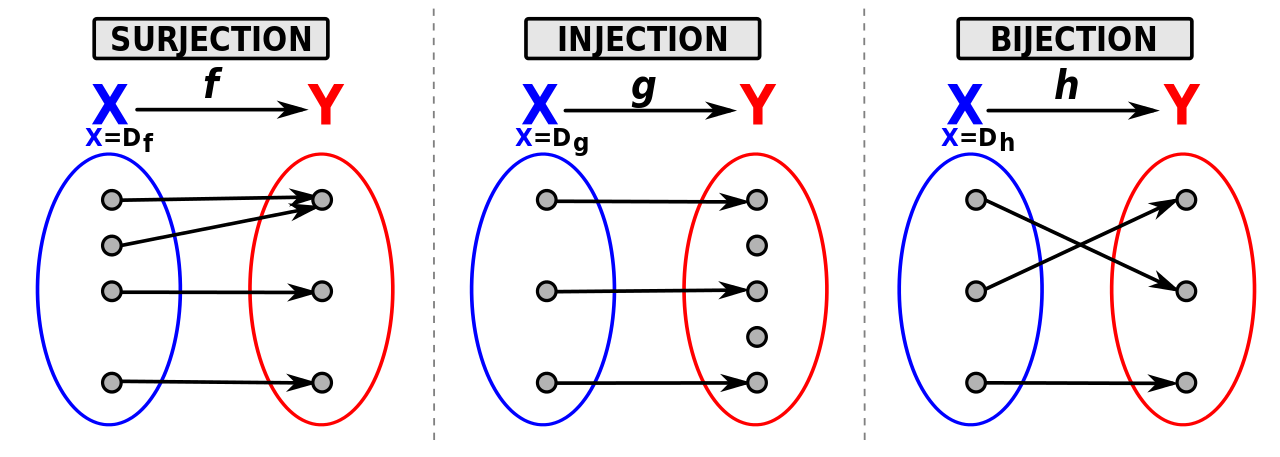
\includegraphics[scale=0.25]{images/fonctions.png}
\begin{itemize}
\item[Injective] one-on-one (many-on-one). $\forall a_1, a_2 \in A, (a_1 \neq a_2) \rightarrow f(a_1) \neq f(a_2)$. Every element of B is hit at most once.
\item[Surjective] $\forall b \in B \exists a \in A f(a) = b$. every b is hit at least once (has at least one pre-image).
\item[Bijective] injective + surjective. $\forall b \in B \exists ! a \in A f(a) = b$
\end{itemize}
Let $f:A \rightarrow B$ be a bijection. Then we can define the inverse function, call it $f^{-1}$, in the following way. 
\begin{equation}
f^{-1} B \rightarrow A, b \in B : f(b) \in A
\end{equation}
Since $f$ is a bijection, $\forall b \in B \exists ! a \in A f(a) = b$. Hence define f(b) to be this unique element.\\
\underline{Well defined ?} Yes, since $a \in A$ and $a$ is unique.\\
$f^{-1} \circ f : A \rightarrow A, \forall a \in A, f^{-1}(f(a)) = a$\\
$f \circ f^{-1} : B \rightarrow B, \forall b \in B, f(f^{-1}(b)) = b$\\

\begin{boite}[0.2]
$f^{-1} \circ f = id_A$\\
$f \circ f^{-1} = id_B$
\end{boite}

\subsubsection{Example}
\underline{Claim :} Let $f : A \rightarrow $ be a function and $f : B \rightarrow A$ be a function so that\\
\fbox{$g \circ f = id_A$  and  $f \circ g = id_B$}\\
\\
Then $f$ and $g$ are bijections and g is the inverse of f and vice-versa.\\
\underline{Proof :}\\
{injectivity of f :} $\forall a_1, a_2 \in A (a_1 \neq a_2) \rightarrow (f(a_1) \neq f(a_2)) \equiv (f(a_1) = f(a_2)) \rightarrow (a_1 = a_2) \equiv \neg q \rightarrow \neg p$\\
{surjectivity of f :} $\forall b\in B, \exists a \in A :f(a) = b$
\subsubsection{Examples :}
$f :\mathbb{R} \rightarrow \mathbb{R}_{\geq 0}, f(x) = x^2$\\
surjective, because $f(-1) = f(1) = 1$, and so not injective.\\
BUT : if we change the domain, it can be injective too :\\ $f : \mathbb{R}_{\geq 0} \rightarrow \mathbb{R}_{\geq 0}$\\
$f(x) = x^2$\\
$g : \mathbb{R}_{\geq 0} \rightarrow \mathbb{R}_{\geq 0}$\\
$g(x) = \sqrt{x}$\\
The inverse is also true : \\
$f : \mathbb{R}_{\leq 0} \rightarrow \mathbb{R}_{\leq 0}$\\
$f(x) = x^2$\\
$f^{-1}(x) = g(x) = -\sqrt{x}$\\
\subsection{Other set properties}
\underline{Definition :} We say that two sets A and B have the same cardinality iff there exists a bijection $f: A \rightarrow B$.\\
\underline{Proof :}(that $|A \cup B| = |A| + |B|$ if $A \cap B = \emptyset$)\\
let $|A| = n$ and $|B| = m$, so $|A| + |B| = n + m$\\
$f: A \rightarrow \{1,...n\}, g : B \rightarrow \{1,...,m\}, f,g$ bijections.\\
\underline{claim :} $h : A \cup B \rightarrow \{1,2,...,m+n\}, h$ bijection.\\
%[    mika]\\
\subsubsection{$\aleph_0$}
$|\mathbb{N}|$ is $\aleph_0$ (aleph null)\\
$f: \mathbb{N}_{\geq 0} \rightarrow \mathbb{N}_{>0}$\\
$f(i) = i + 1$ and $f^{-1} = i-1$
\\
\\
$|\mathbb{Q}| = |\mathbb{N}|$\\
$|\mathbb{Q}| = \{0\} \cup \mathbb{Q}_{>0} \cup \mathbb{Q}_{<0}$\\
$|A| = |\mathbb{N}|, |B| = |\mathbb{N}|$ and $|A \cup B| = |\mathbb{N}|$
\\
\\
$|\mathbb{Z}| = |\mathbb{N}_{\geq 0}|$
\begin{center}
\fbox{\begin{minipage}{0.9\textwidth}
\underline{Definition :} We say that a set is countable if it is finite or there exists a bijection with $\mathbb{N}$.
\end{minipage}}
\end{center}
To map $\mathbb{N} \rightarrow \mathbb{Q}$, we do a tabular
\begin{tabular}{c|ccccccccc}
&1&2&3&4&5&6&7&8\\
\hline
1&$\frac{1}{1}$&$\frac{2}{1}$&$\frac{3}{1}$&$\frac{4}{1}$&$\frac{5}{1}$&$\frac{6}{1}$&$\frac{7}{1}$&$\frac{8}{1}$&...\\
2&$\frac{1}{2}$&$\frac{2}{2}$&$\frac{3}{2}$&$\frac{4}{2}$&$\frac{5}{2}$&$\frac{6}{2}$&$\frac{7}{2}$&$\frac{8}{2}$&...\\
3&$\frac{1}{3}$&$\frac{2}{3}$&$\frac{3}{3}$&$\frac{4}{3}$&$\frac{5}{3}$&$\frac{6}{3}$&$\frac{7}{3}$&$\frac{8}{3}$&...\\
4&$\frac{1}{4}$&$\frac{2}{4}$&$\frac{3}{4}$&$\frac{4}{4}$&$\frac{5}{4}$&$\frac{6}{4}$&$\frac{7}{4}$&$\frac{8}{4}$&...\\
4&$\frac{1}{5}$&$\frac{2}{5}$&$\frac{3}{5}$&$\frac{4}{5}$&$\frac{5}{5}$&$\frac{6}{5}$&$\frac{7}{5}$&$\frac{8}{5}$&...\\
5&$\frac{1}{6}$&$\frac{2}{6}$&$\frac{3}{6}$&$\frac{4}{6}$&$\frac{5}{6}$&$\frac{6}{6}$&$\frac{7}{6}$&$\frac{8}{6}$&...\\
6&$\frac{1}{7}$&$\frac{2}{7}$&$\frac{3}{7}$&$\frac{4}{7}$&$\frac{5}{7}$&$\frac{6}{7}$&$\frac{7}{7}$&$\frac{8}{8}$&...\\
7&$\frac{1}{9}$&$\frac{2}{9}$&$\frac{3}{9}$&$\frac{4}{9}$&$\frac{5}{9}$&$\frac{6}{9}$&$\frac{7}{9}$&$\frac{8}{9}$&...\\
\end{tabular}

\underline{Claim :} The countable union of countable sets is countable.\\
$A_i , i \in \mathbb{N}$, each $A_i$ is countable : $A = \underset{i = 1}{\overset{\infty}{\cup}} A_i$\\
\subsection{Cantor's Diagonalization argument}
\underline{Claim :}$\mathbb{R}$ is not countable\\
\\
\underline{Proof :}$\mathbb{R}_1 = (0,1), \mathbb{R}_1 \subseteq \mathbb{R}$ is not countable.\\
Assume that $\mathbb{R}_1$ is not countable. $f: \mathbb{N} \rightarrow \mathbb{R}_1$ bijection.\\
$\mathbb{R}_1 \ni x_1 = f(1)$\\
$x_2 = f(2)$\\
...\\
$x_i = f(i)$\\
\\Decimal expansion :\\
$x_1 = 0.S_{11}S_{12}S_{13}S_{14}S_{15}S_{16}...$\\
$x_2 = 0.S_{21}S_{22}S_{23}S_{24}S_{25}S_{26}...$\\
...\\
$x_i = 0.S_{i1}S_{i2}.....S_{ii}....$\\
make $\Delta_{ii} \in \{0,...,9\}\setminus\{S_{ii}\}$\\
$0.\Delta_{11}\Delta{22}\Delta{33}...$
\subsection{Sequences}
\begin{center}
	\fbox{\begin{minipage}{0.9\textwidth}
	\underline{Definition :} A sequence is a functio from (a subset of)$\mathbb{N}$ to a set B. $f:\mathbb{N} \rightarrow B$\\
 	Some examples of sequences :
\end{minipage}}
\end{center}
 
\begin{itemize}
	\item 1,2,3,4,5,6,7,... Sequence of natural numbers
	\item 2,3,5,7,11,13,... Sequence of primes
	\item 1,1,2,6,24,... $n!$
	\item 0.1.1.2.3.5.8,.. Fibonacci
\end{itemize}
\begin{center}
	\fbox{\begin{minipage}{0.9\textwidth}
Arithmetic Sequence : $a_i = \alpha + \zeta i, \zeta,\alpha \in \mathbb{R}$\\
Geometric Sequence : $a_i = \alpha \cdot r^i, \alpha,r \in \mathbb{R}$
\end{minipage}}
\end{center}

\underline{Claim :} \\
(I)$\sum_{i=o}^{n} i \overset{?}{=} \frac{k(k+1)}{2} = \begin{pmatrix}
k+1\\
2
\end{pmatrix}$\\
(II)$\sum_{i=o}^{k} r^i \overset{?}{=} \frac{r^{k+1}}{r-1}$

\subsection*{Pigeonhole principle}

If we have m objects to put in n boxes, such as m > n, so There must be at least one box with at least two objects in there !\\
For example, let's take socks, of 3 colors. If we have 4 socks, we will have at least one color with two socks. 
%[Dessin : boites, 2x]

n people, and n boxes, from 0 to n-1. Two cases : $\exists$ a person who shook hands with everybody, or not
.
\subsection*{Special functions}
$\mathbb{R}\rightarrow \mathbb{Z}$
\begin{itemize}
\item[Rounding] $x \rightarrow \ulcorner x\lrcorner$ round to the closest integer (down, 1/2 goes to 0)
\item[Floor function] $x \rightarrow \llcorner x \lrcorner$ map to the largest integer $\leq x$
\item[Ceiling function]$x \rightarrow \ulcorner x\urcorner$ map to the smallest integer $\geq x$
\item[Integer part]$x \rightarrow [x]$ map to integer part
\item[factorial] $\mathbb{N}_{\geq 0} \rightarrow \mathbb{N}, n \rightarrow n! = \overset{n}{\underset{i = 1}{\prod}}i$ and we know that $0! = 1$
\end{itemize}

\section{Algorithms}
\begin{boiteV}{0.9}
\Definition "Finite set of instructions to solve a problem"\\
It usually is in the form $f(n) = c_1n^2+c_2n+c_3$
\end{boiteV}

\subsection{Find maximum}

\underline{Given :} $A = \{_1, a_2, a_3,... a_n\}, a_i \in \mathbb{R}$\\
\underline{Task :}Find a maximum element of A and return its value (perhaps return its index)\\
\underline{Example :} $\{\pi, e, -1, 4, 0.003\}$. let indexes be 1,2,3,4,4. Return value 4, and index 4.\\
\underline{Possible solution :}
\begin{enumerate}
\item Sort in ascending order : \{-1, 0.003, e, $\pi$, 4\}
\item Print out last value
\item Find the index of this value in the original list.
\end{enumerate}
\underline{An other better solution :}
\begin{enumerate}
\item Set $x = a_1$, index = 1
\item Go over all remaining elements. If j\ts{th} element is larger than x, set x  $a_j$, index = j.
\item Print x, index
\end{enumerate}
\underline{Cost of this algorithm: } (n-1) comparisons. storage x, index.\\
we would say that this algorithm has a linear complexity.\\
\underline{Note :} Ignore here the question of how much time one comparison takes.

\subsection{Searching}
Given $A= \{a_1,...a_n\}$, a set of objects.\\
\underline{Task :} Given x, an object, return 0 if $x \not \in A$, return index otherwise so that $x = a_{index}$\\
\underline{Possible solution :}
\begin{enumerate}
\item index = 0
\item Go over all elements, i= 1,...n. 
\item Check if $x = a_1$, if so set index = i
\item Print index
\end{enumerate}
This has a linear complexity.\\

But can we do faster ? Yes, but if set A has a structure. One possible structure: A is sorted

\subsection{Sorting}
Given Set $A = \{a_1,...a_n\}$. Assume that $a_i \in \mathbb{R}$\\
\underline{Task :}Sort A in ascending order.\\
$\{\pi, e, -1, 4, 0.004\} \rightarrow \{-1, 0.003, e, \pi, 4\}$

\subsubsection{Bubble sort}
\underline{For i = n downto 2}\\
"put the largest of al the elements from 4 to i at position i"

\subsection{Size of algorithms}
An algorithms usually is in the form $c_1n^2+c_2+c_3$. But as n is often very big, this is $\approx c_1n^2$\\
The possible sizes are :$\underbrace{1}_{\text{constant}}, \underbrace{\log n}_{\text{logarithmic}} \underbrace{n^d}_{\text{polynomial}} n^d \log n \underbrace{a^n}_{\text{exponential}}, \underbrace{n!}_{\text{fatctorial}}, \underbrace{n^n}$

\subsubsection{Big O}
We say that $f(x), \mathbb{R+} \to \mathbb{R}$ is $O(g(x))$ if $\exists k, C$, such that 
\begin{equation*}
\forall x \geq k  , |f(x)| \leq C|g(x)|
\end{equation*}
$|g(x)|$ is up to a constant factor, eventually an upper bound on $|f(x)|$

\subsubsection{Big-$\Omega$}
We say that $f(x)$ is $\Omega(g(x))$ if $\exists x, C > 0$, such that 
\begin{equation*}
\forall x \geq k, |f(x)| \geq C|g(x)|
\end{equation*}

\subsubsection{Big-$\Theta$}
We say that $f(x)$ is $\Theta(g(x)) \leftrightarrow \{f(x)$ is $O(g(x))\} \wedge \{f(x)$ is $\Omega(g(x)\}$

\subsubsection{Little-o}
We say that $f(x)$ is $o(g(x))$ if $\lim\limits_{x \to +\infty}\frac{|f(x)|}{|g(x)|} = 0$

\subsubsection{Examples}
\underline{Example 1:}\\
$f(n) = 2n^2 + 240 n + 9600$ is $O(n^2)$\\
\underline{Proof :} C = 4 and k = 240 works. $|f(x)| = 2n^2 + 240n + 9600  <leq 4n^2$\\
$2n^2 - 240n - 9600 \geq 0 \Leftrightarrow n \geq 151.6$\\
\\
\underline{Example 2:}\\
$s(n) = 31\sqrt{n}\log n + \sqrt{n}\log_{10} n +167n$ \\
$s(n)$ is $O(n\log n)$\\
\underline{Proof :} $s(n) = 31 \sqrt{n} \log n + n \log_{10}n + 167n \leq 31n \log n + n \frac{\log n}{\log 10} + 167 n \log n \leq \underbrace{199}_\text{31+1+167}n\log n$\\
\\
\underline{Example 3:}\\
$f(n) = 1$. $f(n)$ is $O(g(n)) ?$\\
$g(n) = 75$\\
$|f(n)| = 1 \leq 75 = |g(n)| \to C = 1, k = 0 \Leftrightarrow |f(n)| \leq C|g(n)| \forall n \geq k$\\
\\
\underline{Example 4}\\
$\underbrace{n}_\text{f(n)}$ is $O(\underbrace{n^2}_\text{g(n)})$\\
$|f(n)| = n \leq n^2 = |g(n)|$\\
$n^2$ is NOT $O(n)$\\
$n^2 \leq Cn \Leftrightarrow n \leq C$
$n = \max(c+1,k)$\\
\\
\underline{Example 5}
%[trou mika]
\underline{Example 6}\\
$n!$ is $O(n^n)$\\
$n! = \underbrace{\underbrace{1}_{\leq n}\cdot \underbrace{2}_{\leq n}\cdot 3\cdot 4...\cdot (n-1)\cdot n}_\text{n terms} \leq \underbrace{n\cdot n\cdot n\cdot n...\cdot n}_\text{n terms} = n^n$\\
\\
\underline{Example 8:}\\
$n^n \text{ is NOT } O(n!)$\\
$\exists k, C, \text{ st } n^n \leq C n!$\\
$n! \geq (\frac{n}{e})^ne \Rightarrow n^n \leq (\frac{n}{e})^neC \rightarrow e^n \leq eC \text{ Contradiction !}$\\
\\
\underline{Last Example:}
$\log n! \text{ is } O(n \log n)$\\
%[incomprehensible ! décousu}]\\
\\
\\
\underline{Claim :} $f(x) \text{ is } O(g(x)) \leftrightarrow g(x) \text{ is } \Omega(f(x))$\\
\underline{Proof :} $f(x) \text{ is } O(g(x))$ implies that $g(x) \text{ is } \Omega(G(x))$\\
This means that $\exists k, C$, so that $|f(x)| \leq C|g(x)| \forall x \geq k$\\
if $C > 0$, then this implies $|g(x)| \geq \underbrace{\frac{1}{c}}_{> 0} |f(x)| \forall x \geq k$\\
This implies that $g(x)$ is $\Omega(f(x))$\\
\\
\underline{Example :} $f(x) \text{ is } \overset{?}{\rightarrow} e^{f(x)} \text{ is } O(e^{f(x)})$

\section{Modular arithmetic}
\begin{center}
\fbox{\begin{minipage}{0.9\textwidth}
\underline{Definition :} Let $m \in \mathbb{Z}$. we say that $m$ divides $n, n \in \mathbb{Z}$ if there exists $q$ so that $n = m\cdot q$\\
\\
ways of writing : m divides n : $m|n$
\end{minipage} }
\end{center}
\subsection{Basic facts :}
\begin{enumerate}
\item $\{m|a|\} \wedge \{m|b\} \to m|(a+b)$
\item $m|a \to \forall b \in \mathbb{Z}, m|(a\cdot b)$
\item $\{m|n\} \wedge \{n|a\} \to m|a$
\item $\{m|a\} \wedge \{m|b\} \to \forall s,t \in \mathbb{Z}, m|(as + b t)$
\end{enumerate}
\underline{Proofs :}
\begin{enumerate}
\item [trou mika]
\end{enumerate}
\subsection{Division with remainder}
$m \in \mathbb{Z}$, then for any $n\in\mathbb{Z}$, we can write it in the unique form
\begin{equation*}
n = mq + r1
\end{equation*}
$q,r \in \mathbb{Z}, r \in \{0,...,m-1\}$\\
n dividend\\
m modulus/divisor\\
q quotient\\
r remainder\\

\begin{center}
\fbox{\begin{minipage}{0.9\textwidth}
\underline{Definition :}  Given a modulus $m, m \in \mathbb{Z}_{> 0}$, we say that $a,b \in \mathbb{Z}$ are congruent modulo m if $m|a-b$
\end{minipage} }
\end{center}
What does this mean ? $m|a-b \to a-b = mq, q \in \mathbb{Z} \to a= b + mq$\\
In words, two numbers a and b are congruent modulo m if they differ by a multiple of m\\
\\
\underline{Notation :} we write \textit{a mod m} to denote the remainder of a upon division by m

\subsubsection{Basic properties}
\begin{enumerate}
\item $\{a \equiv b \text{ mod } m\} \wedge \{c \equiv d \text{ m }\} \to \{a+c \equiv b+d \text{ mod } m\}$
\item(a+b) mod m = ((a mod m) + (b mod m)) mod m
\item (a$\cdot$b) mod m = ((a mod m) $\cdot$(b mod m)) mod m
\end{enumerate}

\underline{Example :} $7^{10130134567}$ mod 48 = $7\cdot 7^{10130134566}$ mod 48 = $7\cdot (7^2)^{\frac{10130134566}{2}}$ [trou]

\subsection{Compute powers efficiently}
$a^e$ (mod m)\\
Recall Horner's Rule\\
$fx)=\sum_{i=o}^{L}f_ix^i$  f(a) evoluate the polynomial at $x=a$\\
$f(x)=(((f_L\cdot x + f_{L-1})\cdot x + f_{L-2})\cdot x +... + f_1)\cdot x) + f_0$\\
\underline{complexity :}\\
result = $f_L$\\
for $i = L-1$ downto 0{\\
result = result*a+$f_i$}\\
print result\\
\underline{Note :} if at the end we only want f(0) mod m, then we can apply the mod operation at each step.\\
Let us get back to computing $a^e$\\
$e = \sum_{i=0}^L 2^ie_i$\\
\underline{Example:} 13 = $2^0\cdot 1 + 2^1\cdot 0 + 2^2 \cdot 1 + 2^3 \cdot 1$\\
13 = 1101

[trou waaaaaat?]

\subsection{"Hash" functions}
\begin{itemize}
\item set of obkects, each with unique id, $k \in \mathbb{N}, n$ such objects.
\item m locations ; $m >> n$
\item assign object with identity k to location k mod m
\end{itemize}
This is called the "hash".\\
In order to retrieve object, recompute hash, k mod m, and look at spot k mod m.

\subsubsection{Potential problem}
There can be two keys $k_1$ and $k_2, k_1 \neq k_2$ so that $k_1$ mod m = $k_2$ mod m\\
How many collisions do we expect ?	\\
There is a $\frac{1}{m}$ chance dor collisions of specific pair. There are 
$\begin{pmatrix}
n\\
2
\end{pmatrix}
= \frac{n(n-1)}{2} \sim \frac{n^2}{2}$. Expected \# of collisions $\simeq \frac{n^2}{2m} = 1 \text{ if } n =\sqrt{2m}$

\subsection{Cryptography}
\subsubsection*{Caesar Cipher}
\{a,b,c,...,z\} $\to$ \{0,1,2,3,...,25\} $\iff a \to 0, b \to 1,... z \to 25$\\
\underline{Example :} $\underbrace{"hello"}_{\text{plaintext}} \to \underbrace{fsfresf}_{\text{ciphertext}}$\\
g(n)=n+3\\
to encrypt (letter by letter), we use : $f^{-1}\circ g \circ f$ "hello" becomes "khoor"\\
to decrypt (letter by letter), we use : $f^{-1}\circ g^{-1} \circ f$ "khoor" becomes "hello" again

\subsection{Pseudorandom numbers}
$x_0$ seed, integers\\
$x_{i+1} = (x_ia+c)$mod m\\
a multiplier, c increment, m modulus


\section{Prime numbers}
\begin{boiteV}{0.9}
\underline{Definition :} A prime number is a strictly positive number bigger than 1 that has only 1 and itself as positive divisors
\end{boiteV}
\underline{Fact 1 :} Unique prime factorization.\\
Every integer can we written in a unique (up to order) way as a product of primes\\
\\
\underline{Fact 2 :} Simple Version Euler Lemma.\\
Let p be prime, and $a,b \in \Z$. Then if $p|(a\cdot b)$ then $p|a \vee p|b$\\
\\
\underline{Fact 3 :} Distribution of prime Numbers.\\
$\Pi(x) = \# \{p : p \leq x \wedge p \mbox{ is prime}\}$\\
$\Pi(6) = |\{2,3,5\}| = 3$\\
$\Pi(x) \sim \frac{x}{\log(x)} \to \lim\limits_{x \to \infty} \frac{\Pi}{\frac{x}{\log(x)}} = 1$\\
\underline{Note:} Pick "randomly" an k-bit integer. What is the probability that this number is prime ? $\geq \frac{1}{k}$
\subsection{How to generate a large "random" prime number ?}
\begin{enumerate}
\item Generate a large random number, call it m (Not trivial/easy, we will not see it).
\item Check if m is prime. If yes print, if no go back to 1
\end{enumerate}
We know that we will do this loop about k times (= $\log_2 q$), where k is binary length of desired number
\subsubsection{Lemma}
Let p be prime, S = \{1,2,...p-1\}.\\
Let $a\in S$ and define the map f(x)= $\underline{a\cdot x \mod p}, x  \in S$.\\
1. f: $S\to S$\\
2. f is a bijection\\
\\
\underline{Example :}$ p = 7, S = \{1,2,3,4,5,6\}, a = 3, f(x) = 3\cdot x \mod 7$\\
f(2) = 6, f(5) = 1\\
\\
\underline{Proof :}
\begin{enumerate}
\item A priori, $f(x) \in \{0,1,2,3,\ldots, p-1\}$\\
Assume that for some $x\in S$ this cannot be true.\\
Hence $f(x) = 0$ cannot be true.\\
Hence $f(x) \in S, \forall x \in S$
\item $f: S \to S$ is a bijection\\
$x,y;x \neq y;x,y \in S$\\
$f(x) \neq f(y); 1 \leq x < y \leq p-1$\\
$a\cdot x \not  \equiv a \cdot y \mod p$\\
$a(y-x) \not \equiv 0 \mod p$\\
$y-x \in S$. By 1 indeed $a(y-x) \not \equiv 0 \mod p$
\end{enumerate}

Let p = 7, a = 3.$ ?\exists b \in \{1,2,3,4,5,6\}$ so that $a\cdot b \equiv 1 \mod p$\\
$f^{-1} S \to S; f(f^-1(1)) = f(b)  \equiv ab \mod p$\\
\\
\underline{Claim :} \f is injective implies that \f is also surjective \\
\underline{Proof :} \\
$f : A \to A$ injective\\
$f :A \to f(A)$ injective + surjective $\to$ bijective

\subsection{Commutative Groups}
\subsubsection{(G, + mod p)}
\begin{boiteV}{0.3}
p prime\\
G = \{0,1,\ldots,p-1\}
\end{boiteV}

\begin{enumerate}
\item $a+b \mod p \in G \leftarrow$ closure
\item $((a+b)+c = a+(b+c))\leftarrow$ associativity
\item $a+e \equiv a \mod p; \forall a \in G\leftarrow$ e identity wrt + ; e = 0
\item $a+b \equiv e \equiv 0 \mod p \leftarrow$ b is inverse of a wrt +
\item $a+b \equiv b+a \mod p \leftarrow$ commutativity
\end{enumerate}
We say that (G, + mod p) forms a commutative group
\subsubsection{(G, $\cdot$ mod p)}
\begin{boiteV}{0.35}
$G^* = \{1,2,3,\ldots,p-1\}$\\
$\cdot$ mod p
\end{boiteV}

\begin{enumerate}
\item $a \cdot b \mod p \in G^*\leftarrow$ closure
\item $a\cdot (b \cdot c) \equiv (a\cdot b) \cdot c mod p\leftarrow$ associativity
\item $a\cdot i \equiv 0 \mod p \leftarrow$ i = 1 identity $\surd$
\item $a\cdot b \equiv 1 \mod p\leftarrow$ b is called the inverse wrt $\cdot$ of a
\item $a\cdot b \equiv b \cdot a \mod p \in G \leftarrow$ commutativity
\end{enumerate}
We say that (G, $\cdot$ mod p) is an obelion group (obelion = comutative)
\subsubsection{Distributive law}
$a\cdot(b+c) \equiv a \cdot b +a \cdot c \mod p$\\
($\underbrace{F_p}_{\mbox{field}} = \{0,1,2,\ldots,p-1\}, + \mod p, \cdot \mod p)$
\subsection{Fermat's little Theorem}
Let p be prime. Then $\forall a \in  \Z, a^p \equiv a \mod p$\\
\underline{Proof :} S = \{1,2,\ldots,p-1\} a as given\\
f(x) = ax mod p; $f: S \to S$ is a bijection\\
\underline{Note :} We can assume that $a \in \{0,...,p-1\}$\\
\\
If a = 0, then it's trivially true. It's enough to prove for $a \in S$
$a\cdot \{1,2,3,...,p-1\} = \{1\cdot a, 2\cdot a, 3\cdot a,...,(p-1)\cdot a\} \equiv S \mod p$\\
$\Pi^{p-1}_{i=1} i = \Pi^{p-1}_{i=1}a_i \mod p = a^{p-1}\cdot \Pi^{p-1}_{i=1}i$\\
$(p-1)! = a(p-1)! \mod p$\\
$1 = a^{p-1} \to \underline{a \equiv a^p \mod p}$
\subsection{How to efficiently generate}
Test of Fermat's little theorem :
$2^23 \mod 23 = (2^5)^4\cdot 2^3 \mod 23 = (\underbrace{9^2}_{81})^2 \cdot 2^3 \mod 23 =12^2\cdot2^3 \mod 23 = 24^2\cdot 2 mod 23 = 2 \mod 23$\\

But : $2^{25} \mod 25 = (2^5)^5 \mod 25 = 7^5 \mod 25 = (7^2)^2\cdot 7 \mod 25 = (49)^2 \cdot 7 \mod 25 = (-1)^2 \cdot 7 \mod 25 = 7 \mod 25$. Because 25 is not prime.\\
\\
\underline{Note :} There are numbers, not priume, that pass this test for all $a \in \Z$. These are called pseudo-primes, Cormichael numbers. Example : 561.\\
\\
\underline{Fact :}for large numbers, very few are pseudo-primes.
\subsection{Euclidean Algorithm (gcd)}
\begin{boite}
Let $a,b \in \Z$. Then the gcd of a and b, written gcd(a,b) is the largest positive integer d so that $(d|a)\wedge(d|b)$
\end{boite}
\underline{Example :} gcd(15,125) = 5; 15 = 3x\underline{5}, 125 = \underline{5}x5x5
\underline{Idea :} \underline{Claim :} gcd(a,b) = gcd(a+$\alpha$b), $\forall \alpha \in \Z$\\
\underline{Proof :} \begin{itemize}
\item if $d|a \wedge d|b \to d|b+\alpha a; \forall \alpha \in \Z$
\item if $d|a \wedge d|b+\alpha \to d|a \wedge d|(b+\alpha a) - \alpha a \equiv d|b$. \\
	$\Rightarrow gcd(a,b) = $(because $\leq$(with 1) and $\geq$ (with 2)) $gcd(a, \underbrace{b+\alpha a}_{\equiv b \mod a})$ 
\end{itemize}
\subsubsection{Complexity}
$gcd(a,b) = gcd(|a|,|b|)$. We can assume a,b \\
$gcd(a,b) = gcd(b,\underbrace{a\mod b}_{c})$ (and as $a\geq b \to ) = gcd(b,c)$\\
Claim : $\frac{c}{a} \geq \frac{1}{2}, gcd(c,b)$. Hence, \underline{we need at most $2\log_2 \max(a,b)$ modulo computations}
\subsubsection{Algorithm}
\underline{Theorem :} $\forall a,b \in \Z, \exists \alpha, \delta \in \Z$ so that $gcd(a,b= \alpha a + \delta b$\\
\underline{Proof :} Via extended Euclidean algorithm,\\
$gcd(69,51) =$
\begin{align*}
\fbox{69} =& 1\cdot \fbox{51}+ 18\\
\fbox{51} =& 2\cdot 18 + 15\\
18 =& 1\cdot 15+ 3\\
15 =& 5 \cdot 3  + 0
\end{align*}
Thus, $gcd(69,51) = 3$\\
\\
and, the other way around:
\begin{align*}
18 =& \fbox{69}-\fbox{51}\\
15 = & \fbox{51} - 2 \cdot 18 = \fbox{51}-2\cdot(\fbox{69}-\fbox{51}) = 3 \cdot \fbox{51} - 2\cdot \fbox{69}\\
3 =& 18-15 = \fbox{69}-\fbox{51} - 3 \cdot \fbox{51}+ 2\cdot \fbox{69}\\
&=3\cdot\fbox{69}-4\cdot\fbox{51}
\end{align*}

\paragraph{Why is this useful ?
\underline{Question :} What is the multiplicative inverse of $a \mod b$ ?\\
assume $gcd(a,b) = 1$. By extended Euclidean Algorithm, $\alpha a + \delta b \equiv gcd(a,b) \equiv 1 \mod b \equiv \alpha a (\mbox{ because } \delta b \equiv 0 mod b)$. Easy to show that iff $gcd(a,b) > 1$, a does not have a multiplicative inverse}


\section{Induction}
 P(n). \underline{Example :} P(n) = $"\sum^n_{i=0} i = \frac{n(n+1)}{2}"$\\
 \underline{Aim :} Show that $\forall n \in \mathbb{N}_{\geq 0} P(n)$ is true\\
 \underline{Proof method :}$\underbrace{(P(0)}_{\text{Base Case}} \wedge \underbrace{\forall n \in \mathbb{N}_{\geq 0} P(n) \to P(n+1)}_{\text{Induction Step}}) \Longrightarrow \forall n \in \mathbb{N}_{\geq 0}$\\
 \\
 \underline{Example :} For $n \geq 0, \sum^n_{i=0}i = \frac{n(n+1)}{2}$\\
 We will use mathematical induction to prove this claim.\\
 $P(n) = "\sum^n_{i=0} = \frac{n(n+1)}{2}"$ Want to show that $\forall n \in \mathbb{N}_{\geq 0} P(n)$ is true\\
\underline{Base step :} P(0) true ? $0 = \sum^0_{i=0} \overset{?}{=} \frac{0(0+1)}{2} = 0 \surd$\\
\underline{Induction step :} $\forall n \in \mathbb{N}_{\geq 0} P(n) \to P(n+1)$ is this correct ? $P(n+1) = \sum^{n+1}_{i=0}i = \frac{(n+1)(n+2)}{2} true? \\
\sum^{n+1}_{i=0}i = \sum^{n}_{i=0}i + (n+1) = \frac{n(n+1)}{2} + (n+1) = \frac{n^2+n+2n+2}{2} = \frac{n^2 + 3n + 2}{2} = \frac{(n+1)(n+2)}{2} \surd$\\
\underline{Why correct ?} Proof by contradiction : $p \to q$ and $p \wedge \neg q$ lead to the contradiction
$\underbrace{(P(0) \wedge \forall n \in \mathbb{N}_{\geq 0} P(n) \to P(n+1)}_{\text{assumption p}} \wedge \underbrace{\exists k \in \mathbb{N}_{\geq 0} \neq P(k)}_{\neg q}$\\
Let s be the smallest natural number, $s \in \mathbb{N}_{\geq 0}$ so that P(s) is false. If s = 0, then we are done since we have found our contradiction, since by assumption P(0) is true. If $s > 0$, then by assumption P(s-1) is true, since s was assumed to be the smallest natural number so that P(s) is false. But by the induction step, we know that P(s-1)$\to$P(s), $s-1 \geq 0$. Together with P(s-1) being true, this implies tat P(s) is true, a contradiction.\\
\underline{Note :} Base step is important !\\
\\
\underline{Example :} Claim : $n^3-n$ is divisible by 3 for $n \geq 0$. P(n) = "$3|n^2-n", \forall n \in \mathbb{N}_{\geq 0}$ true\\
\underline{Base step} $P(0) = "3|0" \surd, P(1) = "3|0" \surd$\\
\underline{Induction step} $\forall n \in \mathbb{N}_{\geq 0} P(n) \to P(n+1)$\\
$n(n+1)^3 - (n+1) = n^3-n + 3 (n^2+n) = 0 + 0 = 0 \mod 3 $
\subsection{Strong induction}
$(P(0) \wedge \forall n \in \mathbb{N}_{\geq 0} P(1) \wedge P(2) \wedge P(3)...\wedge P(n) \to P(n+1)) \to \forall n \in \mathbb{N}_{\geq 0} P(n)$
\subsection{mathematical induction}
 $(P(0) \wedge \forall n \in \mathbb{N}_{\geq 0} P(n) \to P(n+1)) \to \forall n \in \mathbb{N}_{\geq 0} P(n)$\\
 Any proof using mathematical induction is still correct if you use induction\\
Assume you have a proof using strong induction for predicate P(n). Consider $Q(n) = P(1) \wedge P(2) \wedge...\wedge P(n)$
\subsection{Tower of Hanoi}
\begin{center}
\includegraphics[scale=0.8]{images/hanoi}
\end{center}
n = 5.\\
n discs on 3 pegs. Discs must be ordered by size on each peg (we can't place a disc on a smaller one)\\
\underline{Aim :} \begin{itemize}
\item Start configuration. Al discs are on  peg 1, sorted
\item bring all discs tot peg 2, again sorted by minimum number of steps. All intermediate configurations must be valid.
\item one step - move one disc
\end{itemize} 
Let C(n) be the minimum number of required steps.\\
\underline{Claim :} "$C(n) \leq 2^n-1" = P(n)$\\
\underline{Proof by induction}\\
 $\underbrace{P(1)}_{\mathclap{\mbox{Base step}}} : C(1) \leq 2^1-1=1 \surd$\\
$\underbrace{P(n) \to P(n+1)}_{\mathclap{\mbox{Induction step}}}\\
C(n) \leq C(n) +1+C(n) = 2C(n) +1 \leq 2(2^n-1)+1 = 2^{n+1}-1\surd$\\
\subsubsection{What is the corresponding algorithm ?}
For a tower of n+1 discs :
\begin{enumerate}
\item Use algorithm for n discs to move the top n discs from peg 1 to peg 3. This can be done in C(n) steps
\item Take the largest disc, which is still on peg 1 and move it to peg 2, this takes one step
\item move the discs on peg 3 to peg 2; this can be done in C(n) steps
\end{enumerate}
\subsection{Recursive algorithm}
\subsubsection{$a^e \mod m$}
\underline{$a^e \mod m$} $(e \geq 0, m \geq 1)$\\
$a^e \mod m = 
\left\{
\begin{array}{ll}
1 & e=0\\
(a^{\frac{e}{2}})^2 & e > 0 \wedge e \mbox{ even}\\
(a^{\lfloor\frac{e}{2}\rfloor})^2a & e \mbox{ odd}
\end{array}
\right.
$
$\underline{\mbox{power } (a, \overbrace{e}^{\geq 0}, \overbrace{m}^{\geq 1})}$ : \\
if e ==0 return  1 mod m;\\
else \{t = power($a, \lfloor\frac{e}{2}\rfloor, m)^2$

if (e is even) return t\\
else return at mod m

[scanner le dessin avec des box]
\subsubsection{n!}
Factorial(n) :\\
If $n \leq 0$ return 1;\\
else return $n\cdot$ factorial(n-1)
\subsubsection{Fibonacci}
$F_n = F_{n-1} + F_{n-2}, n \geq 2$\\
$F_0 = 0, F_1 = 1$\\
0,1,1,2,3,5,8,...\\
fibonacci(n) :\\
if $n \leq 2$ return n;\\
else return fibonacci(n-1) + fibonacci(n-2);
\subsubsection{gcd(a,b)}
gcd(a,b):\\
if b == 0 return a;\\
else return gcd (b, a mod b);
\subsubsection{egcd(a,b)}
(extended)$gcd(ab)$\\
if b == 0 return (a,1,0)\\
else ($d, \alpha, \beta$) = egcd(b, a mod b);
return ($d, \beta, \alpha- \lfloor\frac{a}{b}\rfloor$);

\section{Probabilities}
\subsection{Counting}
Two basic Rules
\begin{enumerate}
	\item \evid{Product rule:} \\
	If a task can be accomplished by first doing task A and then task B, where A can be done in a ways and B in b ways and there is no dependence between A and B, then the overall task can be done in $a\cdot b$ ways
	\item \evid{Sum rule:}\\
	If the task can be accomplished by either doing A \underline{or} B, then the overall task can be done in a+b steps.
\end{enumerate}
\evid{Examples}
Alphabet = \{a,b,c,...,z\} = 26 characters
\begin{enumerate}
	\item How many sequences of length 6 from this alphabet ?\\
	$\overbrace{26}^1\cdot\overbrace{26}^2\cdot\overbrace{26}^3\cdot\overbrace{26}^4\cdot
	\overbrace{26}^5\cdot\overbrace{26}^6 = 26^6$
	\item Sequences that \underline{start} with with a vowel = \{a,e,i,o,u\}\\
	$\overbrace{5}^1\cdot\overbrace{26}^2\cdot\overbrace{26}^3\cdot\overbrace{26}^3\cdot
	\overbrace{26}^5\cdot\overbrace{26}^6\ = 5 \cdot 26^5$
	\item Start and end with a vowel \\
	$\overbrace{5}^1\cdot\overbrace{26}^2\cdot\overbrace{26}^3\cdot\overbrace{26}^3\cdot
	\overbrace{26}^5\cdot\overbrace{5}^6 = 5^2\cdot 26^4$
	\item start or end with a vowel\\
		inclusion-exclusion principle\\
		$\left.
		\begin{tabular}{l}
			\mbox{A all sequences that start with a vowel}\\
			\mbox{B all sequences that end with a vowel}
		\end{tabular}
		\right\} |A\cup B| = |A| + |B| - |A \cap B $\\
		$5\cdot26^5 + 5 \cdot 26^5 - 5^2\cdot26^6 = 26^6 - \underbrace{21^2\cdot26^4}_{\mathclap{\mbox{{sequences that start and end with a consonnant}}}} = 5\cdot 26^4\cdot(2\cdot26-5) (=\alpha_4)$
		\item Sequences that have a vowel at the start or the end, but not both.\\
		V A A A A C $\to 5 \cdot 26^4 \cdot 21$\\
		C A A A A V $\to 21 \cdot 26^4 \cdot 5$\\
		$\to 2 \cdot 5 \cdot 21 \cdot 26^4 = \alpha_4 -21^2\cdot 26^4$
		\item Sequences that have exactly one vowel \\
		$\left.\text{
		\begin{tabular}{lll}
		$A_1$ & a vowel at position 1 & $|A_1| = 5\cdot(21)^5$\\
		$A_2$ & a vowel at position 2 & $|A_2| = 5\cdot(21)^5$\\
		$A_3$ & a vowel at position 3 & $|A_3| = 5\cdot(21)^5$\\
		$A_4$ & a vowel at position 4 & $|A_4| = 5\cdot(21)^5$\\
		$A_5$ & a vowel at position 5 & $|A_5| = 5\cdot(21)^5$\\
		$A_6$ & a vowel at position 6 & $|A_6| = 5\cdot(21)^5$\\
		\end{tabular}}\right\}$
		$= 6\cdot 5 \cdot (21)^5$
\end{enumerate}

\subsection{How many ways are there to pick r objects from a set of size n}
\begin{boiteV}{0.6}
\begin{itemize}
	\item Does order matter ?
	\begin{itemize}
		\item Yes $\to$ permutation
		\item No $\to$ combination
	\end{itemize}
	\item Repetitions allowed ?
\end{itemize}
\end{boiteV}

\subsubsection{Justifications}
\evid{r out of n}
\begin{enumerate}
	\item Permutation without repetition\\
		$P(n,r) = \frac{n(n-1)(n-2)...(n-r+1)(n-r)(n-r-1)...2\cdot1}{(n-r)(n-r-1...2\cdot 1} = $\fbox{$\frac{n!}{(n-r)!}$}
	\item Combination without repetition\\
		$C(n,r)$ = \combi{n}{r}\\
		$C(n,r)\cdot r! = P(n,r) \to C(n,r) = \frac{P(n,r)}{n!} = $\fbox{$\frac{n!}{(n-r)!r!}$}
	\item Permutations \underline{with} repetitions\\
			$\underbrace{n\cdot n \cdot n\cdot n \cdot n\cdot n \cdot .....n\cdot n }_{r \mbox{ times}} =$ \fbox{$n^r$}
	\item Combinations \underline{with} repetitions = \fbox{$\combin{r+n-1}{n-1}$}
\end{enumerate}
\evid{Claim} : 
$\begin{pmatrix}
	n\\
	r
\end{pmatrix}
= 
\begin{pmatrix} 
	n\\ 
	n-1
\end{pmatrix}$\\
\evid{Algebraic} $\begin{pmatrix}
n\\
r
\end{pmatrix}
= \frac{n!}{r!(n-r)!} = \frac{n!}{(n-r)!(n-(n-r))!} = 
\begin{pmatrix}
n\\
n-r
\end{pmatrix}$ [venn's diagrams, showing complements]
\subsection{Some rules}
\subsubsection{Pascal's identity}
\begin{boiteV}{0.65}
$\begin{pmatrix}
n\\
r
\end{pmatrix}
=
\begin{pmatrix}
n-1\\
r
\end{pmatrix}
+
\begin{pmatrix}
n-1\\
r-1
\end{pmatrix}$ for $0 \leq r \leq n$
\end{boiteV}
$= (n-1)!\left(\frac{1}{r!(n-1-r)!}+\frac{1}{(r-1)!(n-r)!}\right)$\\
$= (n-1)!\left(\frac{(n-r)+r}{R!(n-r)!}\right)$\\
$ = \frac{n!}{r!(n-r)!} \surd$

\subsubsection{Powers}
$(x+y)^n = \somme{n}{r=0}{\begin{pmatrix}
	n\\
	r
\end{pmatrix}}
x^ry^{n-r}$\\
$\underbrace{(x+y)(x+y)(x+y).....(x+y)}_{n \times}$\\
$\begin{pmatrix}
	n\\
	0
\end{pmatrix}
y^n + 
\begin{pmatrix}
	n\\
	1
\end{pmatrix}
y^{n-1}x + 
\begin{pmatrix}
	n\\
	2
\end{pmatrix}
y^{n-2}x^2\ldots$\\
\\
\evid{Claim}
$(x+y)^n = (x+y)(x+y)^{n-1}$\\
\evid{Proof}
\underline{Base step} $(x+y)^1 = x+y = \somme{1}{r=0}{\begin{pmatrix}
	1\\
	r
\end{pmatrix}}
x^ry^{1-r} = 1x^1y^0 + 1x^0y^1 \surd$
\underline{Induction step} $n-1 \to P(n-1)$ is true. \\
$\Rightarrow $

$x+y)^n = (x+y)(x+y)^{n-1}$
\begin{align*}
 = (x+y)\somme{n-1}{r=0}{\combin{n-1}{r} x^ry^{n-1-r}} &= \somme{n-1}{r=0} {\combin{n-1}{r} x^{r+1}y^{n-1+r}} + \somme{n-1}{r=0} {\combin{n-1}{r} x^ry^{n-r}}\\
& =x^n+\somme{n-1}{r=1}{\combin{n-1}{r-1} x^ry^{n-r}} + \somme{n-1}{r}{\combin{n-1}{r}x^ry^{n-r}+y^n}
[trou???]
\end{align*}
\subsubsection{Vandermande Identity}
$\combin{m+n}{r} = \somme{r}{k=0}{\combin{n}{r-k}\combin{m}{k}}$ for $0 \leq r \leq m+n$

\subsubsection{Other Rule}
$\combin{n}{r}\combin{r}{k} = \combin{n}{k}\combin{n-k}{r-k}$

\subsection{Some examples}
Let's take a deck of cards : 13 figures (2,3,...,9,10,jack, queen, king, ace) and 4 suits (spades, clubs, heads, diamonds), for a total of 52 cards. Notation : a hand is a set of 5 cards.
\begin{enumerate}

	\item \evid{How many hands are there ?}\\
			$\combi{52}{5} = \frac{52!}{5!(52-5)!} = 2'598'960$
	\item \evid{Hands that contain a specific favourite card}\\
		$\sim \combi{51}{4} = 249'900 \sim 10\%$
	\item $\combi{50}{3}$\\
	A : set of hands \underline{not} containing a\\
	B : set of hands \underline{not} containing b.\\
	$|A\cup B| = |A| + |B| - |A\cap B|$\\
	$\begin{array}{ll}
	|\overline{A\cup B}| & = \text{all}-|A|-|B|+|A\cap B|\\
	& =\combi{52}{5} - \combi{51}{5}-\combi{51}{5} + \combi{50}{5}
	\end{array}$
\end{enumerate}

\subsection{Generating functions}
$F_n = F_{n-1}+F_{n-1}, n \geq 2, F_0 = 0, F_1 = 1$\\
$x^2F_2 = x^2F_1 + x^2F_1$\\
$x^3F_3 = x^3F_2 + x^3F_1$\\
$x^4f_4 = x^4F_3 + x^4F_2$\\
...\\
$x^nF_n = x^nF_{n-1}+x^nF_{n-1}$ And now let's do the sum of all that :\\
$\sum\limits_{i\geq 2} F_ix^i = \sum\limits_{i \geq 1}F_ix^{i+1} + \sum\limits_{i \geq 0}F_ix^{i+2} $\\
\underline{$F(x) = \sum\limits_{i \geq 0}F_ix^i$ is a generating function}\\
$\sum\limits_{i\geq 0}F_ix^{i+2} = x^2\sum\limits_{i\geq 0}F_ix^i = x^2F(x)$\\
$\sum\limits_{i\geq 1}F_ix^{i+1} = x\sum\limits_{i\geq 1}F_ix^i = x\left(\sum\limits_{i\geq 0}F_ix^i-\underbrace{F_0x^0}_{=0}\right) = xF(x)$\\
$\sum\limits_{i\geq 2}F_ix^i = \sum\limits_{i\geq 0}F_ix^i-F_0x^0-F_1x^1 = F(x) - x$\\
$F(x) - x = xF(x) + x^2F(x)$\\
$F(x)\left(1-x-x^2\right) = x$\\
$F(x) = \frac{x}{1-x-x^2}$\\
Let's assume we have something of the form $G(x) = \frac{1}{1-x} = \sum\limits_{i\geq 0} x^1$\\
$G(x) = \frac{1}{1-\alpha x} = \sum\limits_{1 \geq 0} \alpha^ix^1$
We'll attempt to write our function as $F(x) = \frac{x}{1-x-x^2} = -\frac{A}{(x-x_1)} - \frac{B}{(x-x_2)} = \frac{A(x-x_2)+B(x-x_1)}{-x^2+x(x_1+x_2) - x_1x_2}$\\
$-x^2-x+1 = 0$\\
$x_{1,2} = \frac{-b\pm\sqrt{b^2-4ac}}{2a} = \frac{1\pm\sqrt{1+4}}{-2} = \frac{-1\pm\sqrt{5}}{2} \sim -1.6 / 0.6$\\
$x_1 = \frac{-1+\sqrt{5}}{2} ; x_2 = \frac{-1-\sqrt{5}}{2}$\\
.............\\
$F_n = \frac{1}{\sqrt{5}}\left(\left(\frac{2}{\sqrt{5}-1}\right)^n - \left(\frac{2}{-\sqrt{5}-1}\right)^n\right)$
\subsubsection{A new example}
\begin{enumerate}
	\item $f_n = 6 f_{n-1} - 11 f_{n-2} + 6 g_{n-3}, f_0 = 3, f_1 = 6, f_2 = 14$.
	\item "Summing".\\
	$\sum\limits_{n\geq 3}f_nx^n = 6x\sum\limits_{n\geq 2}f_{n-1}x^{n-1} - 11x^2\sum\limits_{n\geq 1}f_{n-2}x^{n-2} + 6x^3\sum\limits_{n\geq 0}f_{n-3}x^{n-3}$
	\item Write in terms of $F(x) = \sum\limits_{n\geq 0} f_ix^i$\\
	$F(x)-f_0-f_1x-f_2x^2 = 6x(F(x)-f_0-f_1x)+11x^2(F(x)-f_0) + 6x^3F(x)$
	\item "Solve" for $F(x)$\\
	$F(x)(1-6x-11x^2-6x^3)=3-12x+11x^2$\\
	$F(x) = \frac{3-12x-11x^2}{1-6x-11x^2-6x^3}$
	\item Write $F(x)$ as a sum of "simple" functions (partial fractions).\\
	$F(x) = \frac{1}{1-x} + \frac{1}{1-2x} + \frac{1}{1-3x}$
	\item Write those "simple"terms as sums.\\
	$F(x) = \sum\limits_{n\geq 0}x^i + \sum\limits_{n\geq 0}2^ix^i + \sum\limits_{n\geq 0}3^ix^i$\\
	$\iff f_n = 1^n+2^n+3^n$.
\end{enumerate}

\subsubsection{Formal Power Sums}
$f_,f_1,f_2,f_3,...$ (infinite, real, complex, whatever) $\iff F(x) = f_0x^0 + f_1x^1 +f_2x^2 +f_3x^3+....$

\subsubsection{Guiding principle} 
\begin{boite}
Any operation is defined as usual as long as for the result the i\ts{th} term is determined by a finite number of operations
\end{boite}
\begin{enumerate}
	\item $f_0,f_1,f_2,... \iff F(x) = f_0 + f_1x^1 + f_2x^2 + f_3x^3+....$\\
	$g_0,g_1,g_2,... \iff G(x) = g_0+g_1x^1+g_2x^2+g_3x^3+....$\\
	$f_0+g_0,f_1+g_1,f_2+g_2,... \iff (f_0+g_0)+(f_1+g_1)x+(f_2+g_2)x^2+(f_3+g_3)x^3.... = F(x) + G(x)$\\
	$\alpha \in \R$\\
	$\alpha f_0,\alpha f_1,\alpha f_2,... \iff (\alpha f_0)+(\alpha f_+)x+(\alpha f_1)x^2+(\alpha f_3)x^3+...=\alpha F(x)$\\
	$F(x) + \underbrace{E(x)}_{\mathclap{\mbox{neutral element}}} = F(x) \iff E(x) = 0 + 0x + 0x^2 +.... 0$\\
	$F(x) + G(x) =E(x) = 0 \iff G(x) = -F(x) = (-f_0) + (-f_1) + ...$
	\item \evid{Shift}\\
	$F_0,f_1,f_2,... \iff F(x) = f_0 + f_1x + f_2x +...$\\
	$0,f_1,f_2.f_3,... \iff 0 + f_0x + f_2x^2 + f_2x^3 + ... $defined as $xF(x)$
	\item \evid{Multiplication}\\
	$F(x)\cdot G(x)$\\
	$(f_0+f_1x+f_2x^2+f_3x^3+...)(g_0+g_1x+g_2x^2+..)$\\
	$\to f_0g_0+f_0g_1x+f_0g_2x^2...+f_1g_0x+f_1g_1x^2 + f_1g_2x^3+...$ The power of the x is equal to the sum of the indexes\\
	$\underbrace{(f_0g_0)x^0}_{h_0} + \underbrace{(f_0g_1+f_1g_0)x}_{h_1} +\underbrace{(f_0g_2+f_+g_1+f_2g_0)x^2}_{h_2} \Rightarrow$
	\begin{boite}[0.4]
		\framecolorbox{red}{white}{$h_n = \somme{n}{i=0}f_iG_{n-i}$} convolution
		\end{boite}
	$F8x)N(x) = F(x) \iff N(x) = 1 + 0x + 0x^2 + 0... = 1$\\
	But does there exists $G(x)$ so that $F(x)G(x) = N(x) = 1$ ? Let's say that $H(x) = F(x)G(x)$, and that $h_n = \somme{n}{i=0}f_ig_{n-i} ; \underbrace{h_0 = , h_n = 0, n \geq 1}_{\mathclap{\mbox{We want possible ?}}}$\\
	$1 = h_0 = f_0g_0 \iff g_0 = \frac{1}{f_0}$ Well defined and unique iff $f_0 \neq 0$\\
	$0 = h_1 = g_0g_1 +f_1g_0$, $f$'s and $g_0$ defined. $ \to $\fbox{$g_1 = \frac{-f_1g_0}{f_0}$} Still defined and unique iff $f \neq 0$\\
	$0 =h_2 = f_0g_2 +f_1g_1+f_2g_0$, everything defined except $g_2 \to$ \fbox{$g_2 = \frac{-f_1g_1-f_2g_0}{f_0}$} well defined and unique iff $f_0 \neq 0$ 
	\begin{boite}
	\framecolorbox{red}{white}{$g_n = \frac{\somme{n}{j=0}f_jg_{n-j}}{f_0}$, $n \geq 1, g_0 = \frac{1}{f_0}$}\\
	\evid{Conclusion :} $F(x)$ has a multiplicative inverse if and only if $f_0 \neq 0$ 
	\end{boite}
\end{enumerate}
\subsubsection{Let's put this in a wonderful example}
$F(x) = 1-x, f_0 = 1,f_1 = -1$\\
$H(x) = G(x)\cdot F(x) = 1$. With our formulas, we find that :\\
$g_0 = \frac{1}{f_0} = 1$\\
$g_1 = \frac{-(f_1g_0)}{f_0} = 1$\\
$g_2 = \frac{-(f_2g_0+f_1g_1)}{f_0} = 1$\\
$g_n = \frac{\somme{n}{j=1}f_jg_{n-j}}{f_0} = \frac{g_{n-1}}{1} = g_{n-1}, n\geq 1$\\
$G(x) = 1+x+x^2+x^3+x^4+...$\\
$F(x) = 1-x$\\
$F(x)G(x) = 1$
[trou]

\subsubsection{Theorem}
Let $\frac{p(xP}{q(x)}$ be given so that $\deg(p(x) < \deg q(x)$ and $q(x) = \produit{n}{i=1}{(x-x_i)^{k_i}}; k_i \in \N_{\geq 1}$ (understood : all $x_i$ are distinct). Further, the roots of $p(x)$ and $q(x)$ are distinct.\\
Then, there exists unique numbers $A_{ij}$ so that
\begin{equation}
	\frac{p(x)}{q(x)} = \somme{n}{i=1}{\somme{k_{i-1}}{j=0}{\frac{A_{ij}}{(x-x_i)^{k_i-j}}}}
\end{equation}
\evid{Example} $F(x) = \frac{x-12x-11x^2}{1-6-11x^2-6x^3} = \frac{p(x)}{q(x)} = \frac{A_{10}}{x-1} + \frac{A_{20}}{x-\frac{1}{2}} + \frac{A_{30}}{x-\frac{1}{3}}$\\
 $\deg p = 2, \deg q = 3$\\
$x_1=1,x_2=\frac{1}{2}, x_3\frac{1}{3}$ (for $k_1=1, k_2=1, k_3=1)$\\
$q(x) = (x-1)(x-\frac{1}{2})(x-\frac{1}{3})$\\
$F(x) = \frac{1+3x}{(x-1)^2} = \frac{A_{10}}{(x-1)^2} + \frac{A_{11}}{(x-1)^1}, x_1=1, k_1=2$

\evid{Proof :} \underline{Claim :} It suffices tu show that there is a unique number A so that 
\begin{equation}
	\frac{p(x)}{q(x)} = \frac{A}{(x-x_1)^{k_1}} + \frac{p^*(x)}{(x-x_1)^{k_1-1}q^*(x)},
\end{equation}	
where $q^*(x) = \frac{q(x)}{(x-x_1)^k_1}$ and where $\deg p^* < k_1-1 + \deg q^*$\\
\underline{Equivalently} \\
$p(x) = Aq^*(x) + p^*(x)(x-x_1)$\\
$\underbrace{p(x) - Aq^*(x)}_{\text{polynomial}} = P^*(x)(x-x_1) \iff$ \begin{align*}
p(x) - Aq^*(x) = 0\\
p(x_1) = AQ^*(x_1) | x=x_1\\
A = \frac{p(x_1)}{q^*(x_+)}
\end{align*}

\subsubsection{How to compute partial fractions efficiently}
\begin{enumerate}
	\item Simple roots (roots of multiplicity 1)\\
	$\frac{p(x)}{q(x)} = \frac{p(x)}{q^*(x)\produit{n}{i=1}{x-x_1}} = \somme{n}{i=1}{\frac{A_i}{x-x_1} + \frac{p*(x)}{q(x)}}$\\
	$p(x) = q^*(x)\somme{n}{i=1}{A_1}\produit{n}{\substack{j=1\\j\neq i}}{x}$
	\item Roots of multiplicity $> 1$, $x^*$ has multiplicity $k > 1$\\
	 $\frac{p(x)}{q(x)} = \somme{k-1}{j=0}{\frac{A_j}{(x-x^*)^{k-j}} + \frac{p^*(x)}{q^*(x)}}$. $\deg p^* < \deg p^*, f^*(x) = \frac{q(x)}{(x-x^*)^k}$\\
	 $p(x) = q^*(x)\somme{k-1}{j=0}{A_j(x-x^*)^j + p^*(x)(x-x^*)^k}$\\
	 And so, $A_0 = \frac{p(x^*)}{q^*(x^*)}$, and in general, $A_j = \left(\frac{p(x)}{q^*(x)}\right)^(j)$ (j\textsuperscript{th} derivative), where $x= x^*$
\end{enumerate}
\subsubsection{Summary with an example}
$F(x) = \frac{1+x+x^2}{(x-1)^2(x-2)} = \frac{p(x)}{q(x)} = \frac{A_0}{(x-2)} + \frac{A_1}{(x-1)^2} + \frac{A_2}{(x-1)}$\\
$A_i$ constants. $A_0 = \frac{p(x)}{q'(x)}|_{x=2} \to q(x) = (x-1)^2(x-2) \to q'(x) = 2(x-1)(x-2)+(x-1)^2 \to A_0 = \frac{7}{1} =7$\\
$A_1 = \frac{1}{0!}\left(\frac{p(x)}{x-2}\right)^{(0)}|_{x=1} = -3$\\
$A_2 = \frac{1}{1!}\left(\frac{p(x)}{x-2}\right)^{(1)}|_{x=1} = \frac{(1+2x)(x-2)-(1+x+x^2)}{(x-2)^2}|_{x=1} = -6$\\
$F(x) = \frac{7}{x-2} -\frac{3}{(x-1)^2} - \frac{6}{x-1} = \frac{-\frac{7}{2}}{1-\frac{1}{2}x} + \frac{6}{(1-x)} - \frac{3}{(1-x)^2} = \frac{-7}{2}\sum\limits_{n\geq 0}(\frac{1}{2})^nx^n + 6\sum\limits_{n \geq 0}x^n -3\sum\limits_{n \geq 0}(n+1)x^n = \sum\limits_{n \geq 0}\left(-\frac{7}{2}( \frac{1}{2})^n + 6 - 3(n+1)\right) ; F_n = -(\frac{7}{2})(\frac{1}{2})^n-3(n-1)$\\
\evid{Aside :} \\
$\frac{1}{(1-x)^k} = \sum\limits_{n \geq 0}\combin{n+k-1}{n}x^n$; For example : $\frac{1}{(1-x)^2} = \sum\limits_{n \geq 0}\combin{n+1}{n}x^n = \sum\limits_{n \geq 0}\combin{n+1}{1}x^n = \sum\limits_{n \geq 0}(n11)x^n$\\
\underline{Note:} $\frac{1}{(1-x)^k} = \frac{1}{(k-1)!}(\frac{1}{1-x)})^{(k-1)}$\\
\underline{Proof} $\frac{1}{1-x} = \sum\limits_{n \geq 0}x^n$\\
$\frac{1}{(1-x)^2}$ is the derivative. [...??]

\evid{Note} $\frac{p(x)}{q(x)} = \frac{p(x)}{\pi}(x-x_i)^{k_i}$ is $O((\frac{1}{x})^nn^{k-1})$, x = smallest root, k = multiplicity of smallest root.\\
$\circ k_i = 1; $ simple roots.\\
$\frac{p(x)}{q(x)} = \sum \frac{A_i}{x-x_i} = \sum_i - -\frac{\frac{A_i}{x_i}}{1-\frac{1}{x_i}x} = \sum_i\sum_n-(\frac{A_i}{x_i})(\frac{1}{x_i})^nx^n$

\evid{Claim} $\sum\limits_{n\geq 0}x^n\left(\somme{n}{l=0}{F_l}\right) = \sum\limits_{n\geq 0}x^n\left(F_{n+2}-1\right), n\geq 0$\\
Right part : $=\frac{1}{x^2}\sum\limits_{n\geq 2} F_n x^n - \sum\limits_{n\geq 0} 1x^n =$ \fbox{$\frac{F(x)-x}{x^2}-\frac{1}{1-x}$}.
[??---]


\subsection{Combinations with repetitions revisited}
n cookie types\\
r cookies\\
$F(x) = \sum\limits_{n\geq 0} F_r x^r = \frac{1}{(1-x)^n} = \sum\limits_{n\geq 0} \combin{r+n-1}{n-1}x^r$\\
$(1+x+^2+x^3+....)$ coolie type 1\\
$(1+x+^2+x^3+....)$ coolie type 2\\
$(1+x+^2+x^3+....)$ coolie type 3\\
$F_0+F_1x+F_2x^2+F_3x^3+...$


\section{Probabilities}
\subsection{Introduction examples}
\evid{Disease}
at any instant, the disease has a probability of $\frac{1}{4}$ to infect 0,1,2 or 3 people (equivalently)
$\begin{array}{lll}
\frac{1}{4} & 0 & 0\\
\frac{1}{4} & 1 & \frac{1}{4}\\
\frac{1}{4} & 2 & \frac{2}{4}\\
\frac{1}{4} & 3 & \underline{\frac{3}{4}}\\
&&\frac{6}{4}
\end{array}$
Critical value is 1. For more, the disease might expand.

So :
\begin{itemize}
	\item I'm tested positive for a \underline{very rare} disease $\frac{1}{1M}$ people catch it)
	\item The test is 99\% positive
\end{itemize}
$\Rightarrow$ Should i be worried ? We'll answer that later

\evid{Random walk}
I take the ling of integers (\Z), and start at 0. I then flip a coin. If head, i go right (+1), if tail I go left (-1) (1 dimension). We have a strong probability to come back at 0.\\
But ! if we do that in 2D, and use a 4 faces coin (like pyramid), and same rule : depending on the result, i go up, down, right or left. Here, it's totally different, there is a low probability to actually come home.
\subsection{Proof techniques}
Probabilistic method\\
\underline{Shannon} reliable transmission of information:
We have a binary sequence  010100011100111. We write them on a HDD, and want to read them later. But due to some technical imperfections (called noise), a digit might be wrong (like 010??0011100111). You know that something happened, but don't know what: two flipped, two changed, one changed, nothing ? We technically don't know. 

But, we can add a code at the beginning (like 0011) that will be used as a check. We know how to use \evid{error corrections codes}. With that, up to a certain error degree, we can correct.

\subsection{New theorem}
A square, with a sample space, and a countable amount of outcomes samples (like dots in the square). each point has a number, between 0 and 1 (like 0.3, 0.1, 0.00001,...). \\
$p:(S) \to [0,1]$\\
$\sum\limits_{s\in S}p(s) = 1$\\
\\
\evid{Dice}
Let's take a dice : every face has a probability of $\frac{1}{6}$
Experiment : an event E, $E \subset A\\
E =$ outcome is even \{2,4,6\}\\
$E =$ outcome $\geq 5$ \{5,6\}\\
\\
\evid{Cards} A pack of cards of 52 cards. $|S| = 52$, E = outcome, card is an ace = $\frac{4}{52}$\\
\\
\begin{boite}[0.65]
p(E) "probability" that event happens $\overset{\Delta}{=} \sum\limits_{S\in E} p(s)$
\end{boite} 
note : $p:S \to [0,1]$\\
$p(s) \geq 0, \forall s \in S$\\
$\sum\limits_{S\in S} p(s) = 1$\\
\underline{Claim :} For any $E \subset S, 0 \leq p(E) \leq 1$

\evid{Example} Dice :
$E = \{2,4,6\} = $ outcome is even.\\
$p(E) = \sum\limits_{S\in E}p(s) = p(2) + p(4) + p(6) = 3\cdot \frac{1}{6} = \frac{1}{2}$
$\overline{E} = S\setminus E$\\
$p(\overline{E}) = \sum\limits_{s\in \overline{E}}p(s) = 1-p(E)$\\
\\
E and F, two subsets of S that have an intersection.\\
If $A\cap B = \emptyset \to p(A\cap B) = p(A) +p(B)$\\
For a dice : $E = \{2,4,6\}, F = \{4,5,6\}\\
E\cap F = \{4,6\}, E \cup F = \{2,4,5,6\}\\
p(E) = \frac{1}{2}, p(F) = \frac{1}{2}, p(E\cap F) = \frac{2}{6} = \frac{1}{3}\\
p(E\cup F) = \frac{4}{6} = \frac{2}{3} = p(E) + p(F) -p(E\cap F)$
\subsection{Conditional probability}
E,F positive, non-empty, intersection non-empty.\\
\evid{Dice}\\
$E = \{2,4,6\}\\
F = \{4,5,6\}$\\
Given F, (given that outcome is at least 4), what is the probability that outcome is even.
\begin{boite}[0.25]
	$p(E|F) = \frac{p(E\cap F)}{p(F)}$
\end{boite}

\begin{boite}
\subsection{Law of total probability}
$p(E) = p(E\cap F) + p(E\cap \overline{F})$ For any $F\subset S$	\\
$p(E|F)p(F) =p(F|E)p(E)$ Bayes law\\ 
$p(E|F) = p(F|E)\frac{p(E)}{p(F)}$
\end{boite}
\subsection{Examples}
6 independent throws of an unbiased coin. we can have h,h,h,h,h,h / h,h,h,h,h,t / ... / t,t,t,t,t,t $\to |S| = 2^6$\\
$p(s)$ (probability for each to come out) = $\frac{1}{2^6}$\\
now, our event E is ``last coin toss had as outcome ``tail'' '', and our event F is ``the first 5 outcomes were ``head'' '' (only 2 outcomes, h,h,h,h,h,h / h,h,h,h,h,t)\\
$p(E) = 2^5 \cdot \frac{1}{2^6} = \frac{1}{2} (2^5$ possibilities for the 5 first ones, each of a probability $\frac{1}{2^6}$ to happen)\\
$p(E|F) = \frac{p(e\cap F)}{p(F)} = \frac{\frac{1}{2^6}}{2\cdot \frac{1}{2^6}} = \frac{1}{2}$
\begin{boite}
	We say that E and F are independent iff $p(E\cap F) = p(E)p(F)$ or (equivalently) if $p(E|F) = \frac{p(E\cap F)}{p(F)} = p(E)$ (equivalent if $p(F) > 0$)
\end{boite}
\evid{Example} Family with k kids, $k \geq 2$.\\
E = Family has boys \underline{and} girls\\
E = family has at most one boy.\\
All outcomes have same probability. Are E and F independent
\\
\underline{For $k = 2$} (g,g),(g,b),(b,g)(b,b), all $\frac{1}{4}$ probability.\\
$E = \{(g,b),(b,g)\} ; p(E) = \frac{1}{2}$\\
$F = \{(g,b),(b,g)(b,b)\} ; p(F) = \frac{3}{4}$\\
$p(E)p(F) = \frac{3}{8}$\\
$E \cap F$ = \{(g,b),(b,g)\} ; $p(E\cap F) = \frac{1}{2} \neq \frac{3}{8}$\\
\underline{For k = 3} (g,g,g),(g,g,b),.....,(b,b,b), all $\frac{1}{8}$ probability.\\
$E\cap F = \{(g,g,b)(g,b,b)(b,g,g)\} ; p(E\cap F) = \frac{3}{8}$\\
$E = \{(g,g,b),(g,b,g),(b,g,g),(g,b,b),(b,g,b),(b,b,g)\} ; p(E) = \frac{6}{8} = \frac{3}{4}$\\
$F = \{(g,g,g)(g,g,b)(g,b,g)(b,g,g)\} ; p(F) = \frac{1}{2}$\\
$p(E)p(F) = \frac{3}{8} =p(E\cap F) \to$ independent

\subsubsection{Let's retake the disease example}
D : Disease, $\overline{D}$ does not have disease, Y = test positive, $\overline{Y}$ test was negative\\
$p(Y|D)= 0.99, p(\overline{Y}|\overline{D}) = 0.99, p(D) = 0.00001$\\
.....\\
\begin{boite}
	\begin{itemize}
		\item $p(E|F) = \frac{p(E\cap F)}{p(F)} \iff p(E\cap F) = p(E|F)p(F)$
		\item $p(E) = p(E\cap F)+p(E\cap \overline{F})$
		\item $p(E) = p(E|F)p(F) + p(E|\overline{F})p(\overline{F})$
	\end{itemize}
\end{boite}

\subsubsection{The... SPAM FILTER !}
(note: here, S is not a sample space but an event).\\
S spam, $p(s) = \frac{2}{3}, p(\overline{s}= = 1 - p(s) = \frac{1}{3}$\\
p(``opportunity'' $| S) = \frac{1}{10}$\\
p(``opportunity'' $| \overline{S}) = \frac{1}{100}$

We use Bayes Law :p($s|$``opportunity'') = $\frac{p(\text{``opportunity''}|S)p(S)}{p(\text{``opportunity''}}$\\
p(``opportunity'') = $p(opp.|\cap s) + p(opp.| \overline{S}) = p(opp.|s)p(s) + p(opp.|\overline{s})p(s)$
\subsection{Expected value}
If we take a die, and throw it, what is the "average value", we do :\\
$1\cdot\frac{1}{6} +2\cdot\frac{1}{6} +3\cdot\frac{1}{6} +4\cdot\frac{1}{6} +5\cdot\frac{1}{6} +6\cdot\frac{1}{6} = \frac{7}{2}$\\
$\mathbb{E} [X] =$ expected value
\begin{boite}
\evid{A random variable}\\
A random variable is a map from a sample space to the \R
\end{boite}
\evid{Example : dice} \\
We throw a pair of dice. Our sample space S = \{(1,1), (1,2),\ldots,(6,6)\} (36 possibilities). Each outcome -(3,5) for example- has a probability $\frac{1}{36}$ to happen.\\
Some natural random variables :\\
$X_1 : S \to \R, X_1(s) = s_1$ outcome of the first die ($X_1((3,5)) = 3)$\\
$X_2 : S \to \R, X_2(s) = s_2$ outcome of the second die ($X_2((3,5)) =5$)\\
\line(1,0){100}\\
$X :  S \to \R, X(s) = s_1+s_2$ outcome of the sum of dice $(X((3,5)) = 8$)\\
\\
For $X_+$, all elements (1,1), (1,2), \ldots , (1,6) will result in 1. p($x_1 = 1 = \frac{1}{6} = \sum\limits_{X_1(s) = 1} p(s)$ , and grosso modo the same for $X_2$.\\
Thus, the probabilities are : 
$\begin{array}{llll}
2 : \frac{1}{36} & 3 : \frac{2}{36} & 4 : \frac{3}{36} & 5 : \frac{4}{36}\\
6 : \frac{5}{36} & 7 : \frac{6}{36} & 8 : \frac{5}{36} & 9 : \frac{4}{36}\\
10 : \frac{3}{36} & 11 : \frac{2}{36} & 12 : \frac{1}{36}&
\end{array}$\\
$\to \mathbb{E} [X] = \sum\limits_{r}p(x=r)\cdot r = \sum\limits_r \sum\limits_{s:X(s) = r} r\cdot p(s) = \sum X(s)p(s)$\\
\\
We defined $X(s) = X_1(s) +X_2(s)$, this applies too for the probabilities : \\
$\mathbb{E} [X] = \sum\limits_{s\in S} X(s) p(s) \to \mathbb{E}[X_1+X_2] = \sum\limits_{s\in S} (X_1(s) + X_2(s)) p(s) = \sum\limits_{s\in S} X_1(s) p(s) + \sum\limits_{s\in S} X_2(s) p(s) = \mathbb{E}[X_1] + \mathbb{E}[X_2]$
\subsection{Something else ?}
\begin{boite}
	\evid{Theorem} If X and Y are independent, then 
	\begin{equation}
		\mathbb{E}[X\cdot Y] = \mathbb{E}[X]\cdot \mathbb{E}[Y]
	\end{equation}
	\evid{Definition}
	X and Y are independent if
	\begin{equation}
		p(X=x \wedge Y=y) = p(X=x) \cdot p(Y=y), x,y \in \R
	\end{equation}
\end{boite}
Recall : E,F events.\\
E and F are independent if $p(E\cap F) = p(E)p(F)$\\
$E= \{s\in S : X(s) = x\}$\\
$F= \{s\in S : Y(s) = y\}$
$\to p(X=x) = p(E), p(Y=y) = p(F), P(X=x \wedge Y=y) = p(E\cap F)$\\
\evid{Bernoulli trials :} individual trials are \underline{independent}\\

\subsection{Markov}
Let X be a random variable that is non-negative\\
$\E[X] = \sum\limits_{s\in S} \geq \sum\limits_{\substack{s\in S \\ |X(s)| \geq \alpha}} X(s) p(s) \geq \sum\limits_{\substack{s\in S \\ |X(s)| \geq \alpha}} \alpha p(s) = \alpha \sum\limits_{\substack{s\in S \\ |X(s)| \geq \alpha}}p(s)$
$to$
\begin{boite}
	\begin{equation}
		p(x\geq \alpha) \leq \frac{\E[X]}{\alpha}
	\end{equation}
\end{boite}

\subsection{Chebyshev}
$\underbrace{\E[(X-E[X])^2]}_{\text{variance}} = \sum\limits_{s\in S}(X(s) - \overline{X})^2 p(s)  \geq \sum\limits_{\substack{s\in S \\ |X(s) - \overline{X}| \geq \alpha}} (X(s) - \overline{X})^2 p(s) \geq \alpha^2\sum\limits_{|X(s)-\overline{X}| \geq \alpha} p(s) = \alpha^2 p(|X-\overline{X}| \geq \alpha)$  
\begin{boite}
	\begin{equation}
	p(|X-\overline{X}| \geq \alpha) \leq \frac{\E[(X-\overline{X})^2]}{\alpha^2}
	\end{equation}
\end{boite}


\section{Rules}
\subsection{Logic}
\subsection{Sets}
\begin{itemize}
	\item $|P(A)| = 2^{|A|}$
	\item $|A \times B| = |A| \cdot |B|$ (cartesian product)
	\item $|A \cup B| = |A| + |B| - |A \cap B|$
	\item $|A \cup B \cup C| = |A| + |B| +  |C| - |A \cap B| - |A \cap C| - |B \cap C| + |A \cap B \cap C|$ 
	\item $|A| = |B| \leftrightarrow f: A \rightarrow B$ such as f is a \underline{bijection}
	\item $|A| \leq |B| \leftrightarrow g: A \rightarrow B$ such as f is \underline{injective}
	\item $|B| \leq |A| \leftrightarrow h: B \rightarrow A$ such as f is a \underline{injective}
	\item $|\N \times \Q| = |\N|$
\end{itemize}

\subsection{Counting/Probability}
\begin{itemize}
	\item Combination. We may not pick everybody. We n available case, we chose r.	Order does \underline{not} matter. Just how many way of picking.
		\begin{itemize}
			\item Without repetition : choosing r winners out of n people ($r \leq n$)\\
			 $\combi{n}{r} = \frac{n!}{(n-r)!r!}$
			 \item With repetitions : choosing r cookies to eat out of n sorts (r can be greater than n)\\
			 $\combi{r+n-1}{n-1} =\frac{(r+n-1)!}{((r+n-1)-(n-1))!(n-1)!} = \frac{(r+n-1)!}{r!(n-1)!}$
		\end{itemize}
	\item Permutation. We want to put objects in a specific order. Order \underline{does} matter.
		\begin{itemize}
			\item With repetitions :
		\end{itemize}
\end{itemize}
\subsection{Generating Functions}
\begin{itemize}
	\item $\sum\limits_{n\geq 1} \alpha^n = \frac{\alpha}{1-\alpha}$
	\item $10+9+8+..+1 = 55  = \combi{11}{2}$
\end{itemize}
\section{Glossary}
\subsection{Logic}
\begin{enumerate}
\item[Proposition]
\item[Predicate] P(x)
\item[Quantifier]
\item[Tautology] Proposition that always have a truth value \bo{T}, whatever is the value of it's component
\end{enumerate}
\subsection{Sets}
\begin{itemize}
\item[$P(A)$] Powerset of A. All possible combinations
\item [$\dot{\cup}$] disjoint union
\item [$B \setminus A$] B minus A. We take off B every element of A = $B - (B \cap A)$
\item [$f : A \rightarrow B$] For such a function, A is the \underline{Domain} and B the \underline{co-domain}
\end{itemize}
\subsection{Primes}
\begin{itemize}
\item[$p|a$] p divides a $\to \frac{a}{p} \in \N \to a \mod p = 0$
\end{itemize}
\end{document}